\documentclass[1p]{elsarticle_modified}
%\bibliographystyle{elsarticle-num}

%\usepackage[colorlinks]{hyperref}
%\usepackage{abbrmath_seonhwa} %\Abb, \Ascr, \Acal ,\Abf, \Afrak
\usepackage{amsfonts}
\usepackage{amssymb}
\usepackage{amsmath}
\usepackage{amsthm}
\usepackage{scalefnt}
\usepackage{amsbsy}
\usepackage{kotex}
\usepackage{caption}
\usepackage{subfig}
\usepackage{color}
\usepackage{graphicx}
\usepackage{xcolor} %% white, black, red, green, blue, cyan, magenta, yellow
\usepackage{float}
\usepackage{setspace}
\usepackage{hyperref}

\usepackage{tikz}
\usetikzlibrary{arrows}

\usepackage{multirow}
\usepackage{array} % fixed length table
\usepackage{hhline}

%%%%%%%%%%%%%%%%%%%%%
\makeatletter
\renewcommand*\env@matrix[1][\arraystretch]{%
	\edef\arraystretch{#1}%
	\hskip -\arraycolsep
	\let\@ifnextchar\new@ifnextchar
	\array{*\c@MaxMatrixCols c}}
\makeatother %https://tex.stackexchange.com/questions/14071/how-can-i-increase-the-line-spacing-in-a-matrix
%%%%%%%%%%%%%%%

\usepackage[normalem]{ulem}

\newcommand{\msout}[1]{\ifmmode\text{\sout{\ensuremath{#1}}}\else\sout{#1}\fi}
%SOURCE: \msout is \stkout macro in https://tex.stackexchange.com/questions/20609/strikeout-in-math-mode

\newcommand{\cancel}[1]{
	\ifmmode
	{\color{red}\msout{#1}}
	\else
	{\color{red}\sout{#1}}
	\fi
}

\newcommand{\add}[1]{
	{\color{blue}\uwave{#1}}
}

\newcommand{\replace}[2]{
	\ifmmode
	{\color{red}\msout{#1}}{\color{blue}\uwave{#2}}
	\else
	{\color{red}\sout{#1}}{\color{blue}\uwave{#2}}
	\fi
}

\newcommand{\Sol}{\mathcal{S}} %segment
\newcommand{\D}{D} %diagram
\newcommand{\A}{\mathcal{A}} %arc


%%%%%%%%%%%%%%%%%%%%%%%%%%%%%5 test

\def\sl{\operatorname{\textup{SL}}(2,\Cbb)}
\def\psl{\operatorname{\textup{PSL}}(2,\Cbb)}
\def\quan{\mkern 1mu \triangleright \mkern 1mu}

\theoremstyle{definition}
\newtheorem{thm}{Theorem}[section]
\newtheorem{prop}[thm]{Proposition}
\newtheorem{lem}[thm]{Lemma}
\newtheorem{ques}[thm]{Question}
\newtheorem{cor}[thm]{Corollary}
\newtheorem{defn}[thm]{Definition}
\newtheorem{exam}[thm]{Example}
\newtheorem{rmk}[thm]{Remark}
\newtheorem{alg}[thm]{Algorithm}

\newcommand{\I}{\sqrt{-1}}
\begin{document}

%\begin{frontmatter}
%
%\title{Boundary parabolic representations of knots up to 8 crossings}
%
%%% Group authors per affiliation:
%\author{Yunhi Cho} 
%\address{Department of Mathematics, University of Seoul, Seoul, Korea}
%\ead{yhcho@uos.ac.kr}
%
%
%\author{Seonhwa Kim} %\fnref{s_kim}}
%\address{Center for Geometry and Physics, Institute for Basic Science, Pohang, 37673, Korea}
%\ead{ryeona17@ibs.re.kr}
%
%\author{Hyuk Kim}
%\address{Department of Mathematical Sciences, Seoul National University, Seoul 08826, Korea}
%\ead{hyukkim@snu.ac.kr}
%
%\author{Seokbeom Yoon}
%\address{Department of Mathematical Sciences, Seoul National University, Seoul, 08826,  Korea}
%\ead{sbyoon15@snu.ac.kr}
%
%\begin{abstract}
%We find all boundary parabolic representation of knots up to 8 crossings.
%
%\end{abstract}
%\begin{keyword}
%    \MSC[2010] 57M25 
%\end{keyword}
%
%\end{frontmatter}

%\linenumbers
%\tableofcontents
%
\newcommand\colored[1]{\textcolor{white}{\rule[-0.35ex]{0.8em}{1.4ex}}\kern-0.8em\color{red} #1}%
%\newcommand\colored[1]{\textcolor{white}{ #1}\kern-2.17ex	\textcolor{white}{ #1}\kern-1.81ex	\textcolor{white}{ #1}\kern-2.15ex\color{red}#1	}

{\Large $\underline{12a_{0705}~(K12a_{0705})}$}

\setlength{\tabcolsep}{10pt}
\renewcommand{\arraystretch}{1.6}
\vspace{1cm}\begin{tabular}{m{100pt}>{\centering\arraybackslash}m{274pt}}
\multirow{5}{120pt}{
	\centering
	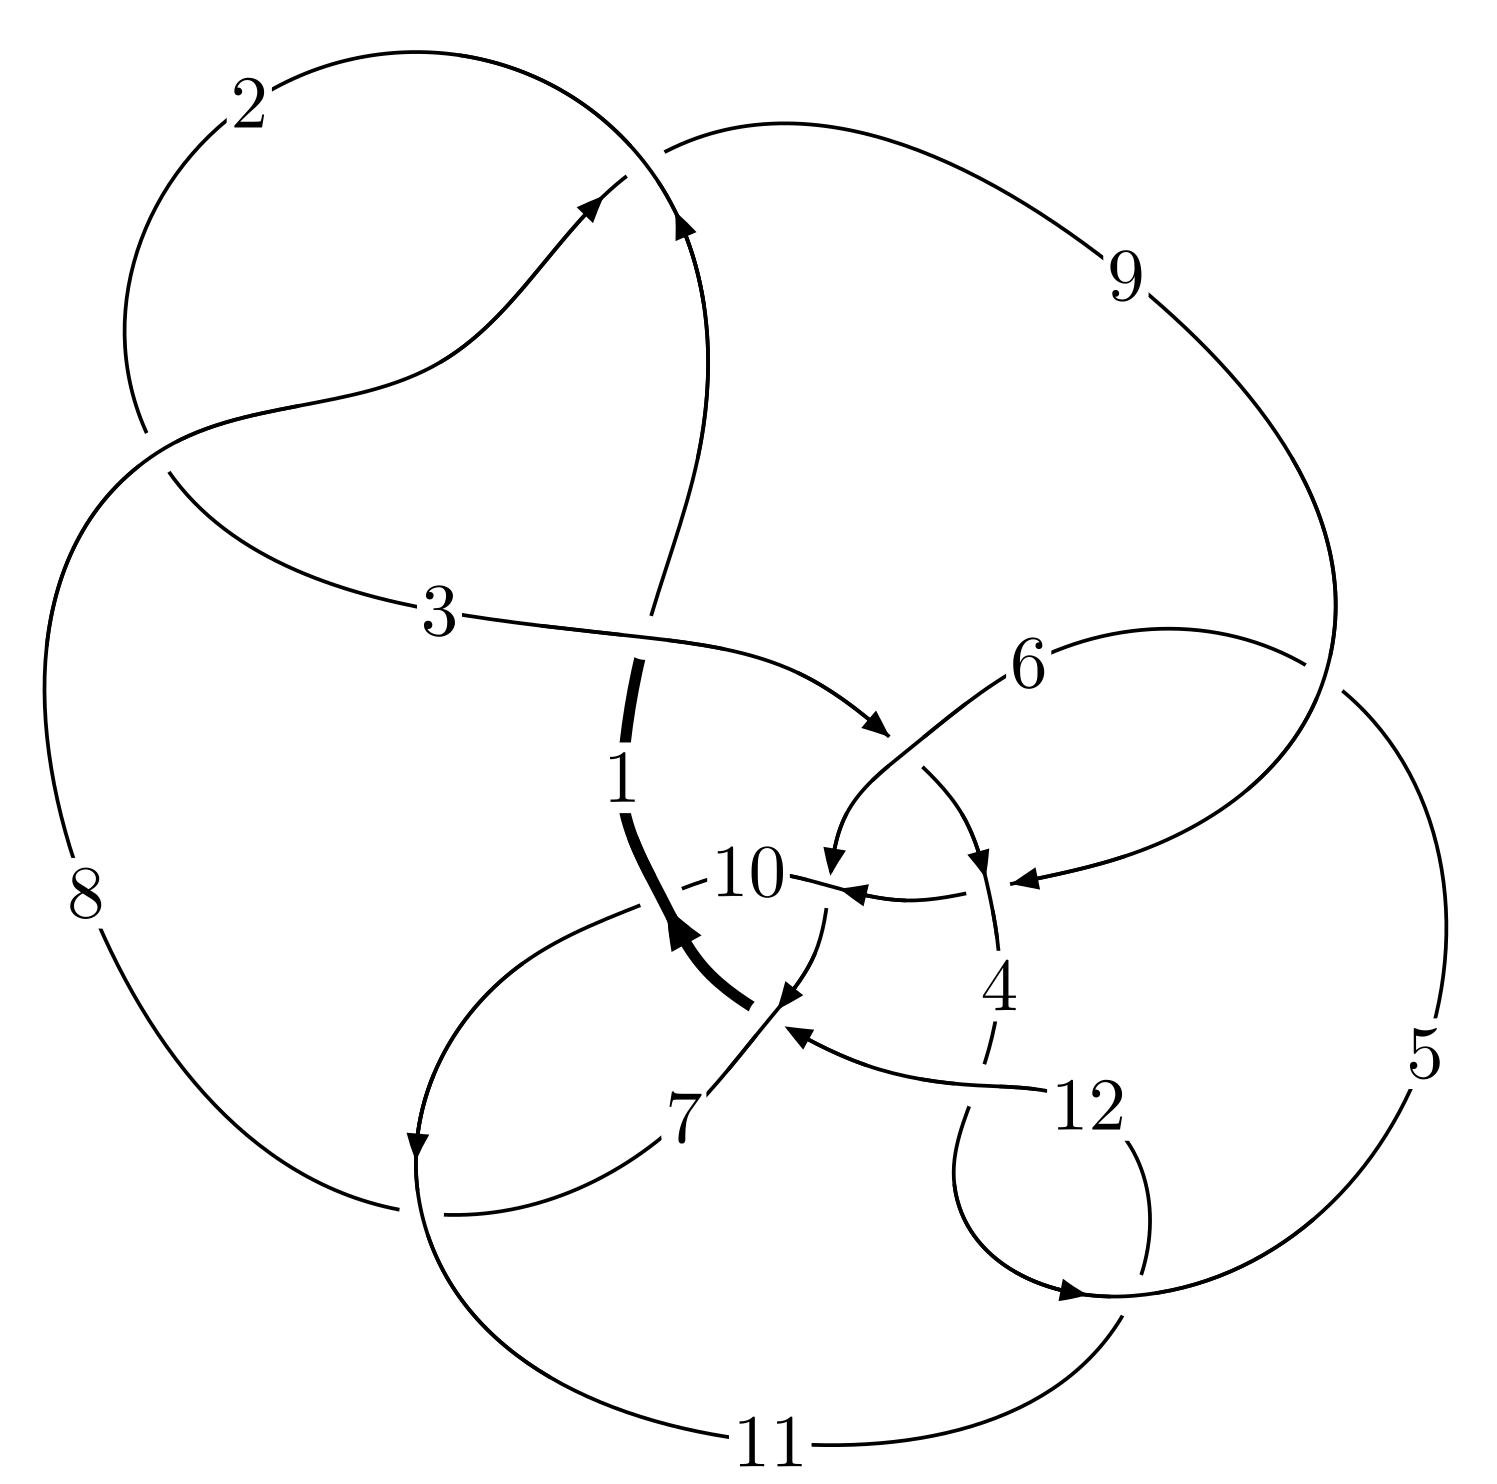
\includegraphics[width=112pt]{../../../GIT/diagram.site/Diagrams/png/1506_12a_0705.png}\\
\ \ \ A knot diagram\footnotemark}&
\allowdisplaybreaks
\textbf{Linearized knot diagam} \\
\cline{2-2}
 &
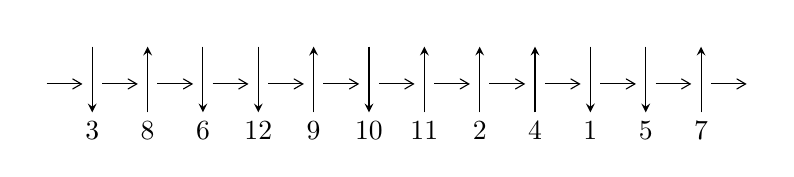
\begin{tikzpicture}[x=20pt, y=17pt]
	% nodes
	\node (C0) at (0, 0) {};
	\node (C1) at (1, 0) {};
	\node (C1U) at (1, +1) {};
	\node (C1D) at (1, -1) {3};

	\node (C2) at (2, 0) {};
	\node (C2U) at (2, +1) {};
	\node (C2D) at (2, -1) {8};

	\node (C3) at (3, 0) {};
	\node (C3U) at (3, +1) {};
	\node (C3D) at (3, -1) {6};

	\node (C4) at (4, 0) {};
	\node (C4U) at (4, +1) {};
	\node (C4D) at (4, -1) {12};

	\node (C5) at (5, 0) {};
	\node (C5U) at (5, +1) {};
	\node (C5D) at (5, -1) {9};

	\node (C6) at (6, 0) {};
	\node (C6U) at (6, +1) {};
	\node (C6D) at (6, -1) {10};

	\node (C7) at (7, 0) {};
	\node (C7U) at (7, +1) {};
	\node (C7D) at (7, -1) {11};

	\node (C8) at (8, 0) {};
	\node (C8U) at (8, +1) {};
	\node (C8D) at (8, -1) {2};

	\node (C9) at (9, 0) {};
	\node (C9U) at (9, +1) {};
	\node (C9D) at (9, -1) {4};

	\node (C10) at (10, 0) {};
	\node (C10U) at (10, +1) {};
	\node (C10D) at (10, -1) {1};

	\node (C11) at (11, 0) {};
	\node (C11U) at (11, +1) {};
	\node (C11D) at (11, -1) {5};

	\node (C12) at (12, 0) {};
	\node (C12U) at (12, +1) {};
	\node (C12D) at (12, -1) {7};
	\node (C13) at (13, 0) {};

	% arrows
	\draw[->,>={angle 60}]
	(C0) edge (C1) (C1) edge (C2) (C2) edge (C3) (C3) edge (C4) (C4) edge (C5) (C5) edge (C6) (C6) edge (C7) (C7) edge (C8) (C8) edge (C9) (C9) edge (C10) (C10) edge (C11) (C11) edge (C12) (C12) edge (C13) ;	\draw[->,>=stealth]
	(C1U) edge (C1D) (C2D) edge (C2U) (C3U) edge (C3D) (C4U) edge (C4D) (C5D) edge (C5U) (C6U) edge (C6D) (C7D) edge (C7U) (C8D) edge (C8U) (C9D) edge (C9U) (C10U) edge (C10D) (C11U) edge (C11D) (C12D) edge (C12U) ;
	\end{tikzpicture} \\
\hhline{~~} \\& 
\textbf{Solving Sequence} \\ \cline{2-2} 
 &
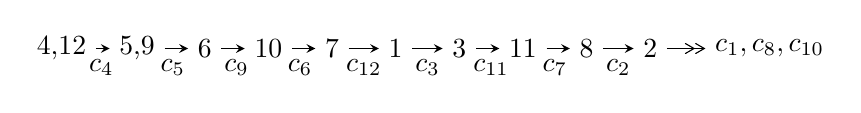
\begin{tikzpicture}[x=23pt, y=7pt]
	% node
	\node (A0) at (-1/8, 0) {4,12};
	\node (A1) at (17/16, 0) {5,9};
	\node (A2) at (17/8, 0) {6};
	\node (A3) at (25/8, 0) {10};
	\node (A4) at (33/8, 0) {7};
	\node (A5) at (41/8, 0) {1};
	\node (A6) at (49/8, 0) {3};
	\node (A7) at (57/8, 0) {11};
	\node (A8) at (65/8, 0) {8};
	\node (A9) at (73/8, 0) {2};
	\node (C1) at (1/2, -1) {$c_{4}$};
	\node (C2) at (13/8, -1) {$c_{5}$};
	\node (C3) at (21/8, -1) {$c_{9}$};
	\node (C4) at (29/8, -1) {$c_{6}$};
	\node (C5) at (37/8, -1) {$c_{12}$};
	\node (C6) at (45/8, -1) {$c_{3}$};
	\node (C7) at (53/8, -1) {$c_{11}$};
	\node (C8) at (61/8, -1) {$c_{7}$};
	\node (C9) at (69/8, -1) {$c_{2}$};
	\node (A10) at (11, 0) {$c_{1},c_{8},c_{10}$};

	% edge
	\draw[->,>=stealth]	
	(A0) edge (A1) (A1) edge (A2) (A2) edge (A3) (A3) edge (A4) (A4) edge (A5) (A5) edge (A6) (A6) edge (A7) (A7) edge (A8) (A8) edge (A9) ;
	\draw[->>,>={angle 60}]	
	(A9) edge (A10);
\end{tikzpicture} \\ 

\end{tabular} \\

\footnotetext{
The image of knot diagram is generated by the software ``\textbf{Draw programme}" developed by Andrew Bartholomew(\url{http://www.layer8.co.uk/maths/draw/index.htm\#Running-draw}), where we modified some parts for our purpose(\url{https://github.com/CATsTAILs/LinksPainter}).
}\phantom \\ \newline 
\centering \textbf{Ideals for irreducible components\footnotemark of $X_{\text{par}}$} 
 
\begin{align*}
I^u_{1}&=\langle 
2.77814\times10^{223} u^{84}+1.16049\times10^{224} u^{83}+\cdots+5.71791\times10^{224} b-2.02352\times10^{225},\\
\phantom{I^u_{1}}&\phantom{= \langle  }6.93165\times10^{224} u^{84}+8.28583\times10^{225} u^{83}+\cdots+4.57433\times10^{226} a+1.25867\times10^{228},\\
\phantom{I^u_{1}}&\phantom{= \langle  }u^{85}+5 u^{84}+\cdots+951 u+160\rangle \\
I^u_{2}&=\langle 
2.63966\times10^{86} a u^{58}+8.74141\times10^{84} u^{58}+\cdots-5.15249\times10^{85} a-6.04873\times10^{86},\\
\phantom{I^u_{2}}&\phantom{= \langle  }5.11511\times10^{86} a u^{58}+5.45554\times10^{85} u^{58}+\cdots-5.67633\times10^{84} a-9.66817\times10^{86},\;u^{59}- u^{58}+\cdots-2 u+1\rangle \\
I^u_{3}&=\langle 
4325521 u^{21} a-5569352 u^{21}+\cdots+770633 a+20960753,\\
\phantom{I^u_{3}}&\phantom{= \langle  }51468579 u^{21} a+49951560 u^{21}+\cdots-135794681 a-49237463,\;u^{22}+13 u^{20}+\cdots-3 u+1\rangle \\
I^u_{4}&=\langle 
- u^4-2 u^3-2 u^2+b-2 u,\;u^4+u^3+a- u-2,\;u^5+2 u^4+3 u^3+3 u^2+u+1\rangle \\
\\
\end{align*}
\raggedright * 4 irreducible components of $\dim_{\mathbb{C}}=0$, with total 252 representations.\\
\footnotetext{All coefficients of polynomials are rational numbers. But the coefficients are sometimes approximated in decimal forms when there is not enough margin.}
\newpage
\renewcommand{\arraystretch}{1}
\centering \section*{I. $I^u_{1}= \langle 2.78\times10^{223} u^{84}+1.16\times10^{224} u^{83}+\cdots+5.72\times10^{224} b-2.02\times10^{225},\;6.93\times10^{224} u^{84}+8.29\times10^{225} u^{83}+\cdots+4.57\times10^{226} a+1.26\times10^{228},\;u^{85}+5 u^{84}+\cdots+951 u+160 \rangle$}
\flushleft \textbf{(i) Arc colorings}\\
\begin{tabular}{m{7pt} m{180pt} m{7pt} m{180pt} }
\flushright $a_{4}=$&$\begin{pmatrix}1\\0\end{pmatrix}$ \\
\flushright $a_{12}=$&$\begin{pmatrix}0\\u\end{pmatrix}$ \\
\flushright $a_{5}=$&$\begin{pmatrix}1\\u^2\end{pmatrix}$ \\
\flushright $a_{9}=$&$\begin{pmatrix}-0.0151534 u^{84}-0.181137 u^{83}+\cdots-148.935 u-27.5159\\-0.0485866 u^{84}-0.202956 u^{83}+\cdots+5.73116 u+3.53891\end{pmatrix}$ \\
\flushright $a_{6}=$&$\begin{pmatrix}0.229002 u^{84}+1.05119 u^{83}+\cdots-12.0998 u-14.1719\\-0.0683057 u^{84}-0.350783 u^{83}+\cdots-74.6193 u-11.0319\end{pmatrix}$ \\
\flushright $a_{10}=$&$\begin{pmatrix}-0.0637400 u^{84}-0.384094 u^{83}+\cdots-143.204 u-23.9770\\-0.0485866 u^{84}-0.202956 u^{83}+\cdots+5.73116 u+3.53891\end{pmatrix}$ \\
\flushright $a_{7}=$&$\begin{pmatrix}-0.0221182 u^{84}-0.159178 u^{83}+\cdots-94.1381 u-15.3032\\-0.0653935 u^{84}-0.272677 u^{83}+\cdots+36.6397 u+10.1984\end{pmatrix}$ \\
\flushright $a_{1}=$&$\begin{pmatrix}0.00497274 u^{84}+0.114466 u^{83}+\cdots+130.312 u+22.5502\\0.0447022 u^{84}+0.202464 u^{83}+\cdots+16.4799 u-0.834762\end{pmatrix}$ \\
\flushright $a_{3}=$&$\begin{pmatrix}-0.104846 u^{84}-0.302981 u^{83}+\cdots+245.097 u+51.8678\\0.0841183 u^{84}+0.400156 u^{83}+\cdots+54.2721 u+6.26190\end{pmatrix}$ \\
\flushright $a_{11}=$&$\begin{pmatrix}u\\u^3+u\end{pmatrix}$ \\
\flushright $a_{8}=$&$\begin{pmatrix}-0.0189559 u^{84}-0.192940 u^{83}+\cdots-178.497 u-31.7372\\-0.0447255 u^{84}-0.208162 u^{83}+\cdots-1.08021 u+1.69630\end{pmatrix}$ \\
\flushright $a_{2}=$&$\begin{pmatrix}-0.290244 u^{84}-1.22579 u^{83}+\cdots+55.3401 u+25.6354\\0.109881 u^{84}+0.562827 u^{83}+\cdots+120.402 u+17.0715\end{pmatrix}$\\&\end{tabular}
\flushleft \textbf{(ii) Obstruction class $= -1$}\\~\\
\flushleft \textbf{(iii) Cusp Shapes $= -0.514445 u^{84}-2.31397 u^{83}+\cdots-6.34406 u+23.9114$}\\~\\
\newpage\renewcommand{\arraystretch}{1}
\flushleft \textbf{(iv) u-Polynomials at the component}\newline \\
\begin{tabular}{m{50pt}|m{274pt}}
Crossings & \hspace{64pt}u-Polynomials at each crossing \\
\hline $$\begin{aligned}c_{1}\end{aligned}$$&$\begin{aligned}
&u^{85}+45 u^{84}+\cdots-58368 u-4096
\end{aligned}$\\
\hline $$\begin{aligned}c_{2},c_{8}\end{aligned}$$&$\begin{aligned}
&u^{85}+3 u^{84}+\cdots+288 u+64
\end{aligned}$\\
\hline $$\begin{aligned}c_{3},c_{10}\end{aligned}$$&$\begin{aligned}
&u^{85}- u^{84}+\cdots-3 u+1
\end{aligned}$\\
\hline $$\begin{aligned}c_{4},c_{11}\end{aligned}$$&$\begin{aligned}
&u^{85}+5 u^{84}+\cdots+951 u+160
\end{aligned}$\\
\hline $$\begin{aligned}c_{5},c_{7}\end{aligned}$$&$\begin{aligned}
&u^{85}+2 u^{84}+\cdots+54 u-1
\end{aligned}$\\
\hline $$\begin{aligned}c_{6}\end{aligned}$$&$\begin{aligned}
&u^{85}+10 u^{84}+\cdots-35445 u-2194
\end{aligned}$\\
\hline $$\begin{aligned}c_{9},c_{12}\end{aligned}$$&$\begin{aligned}
&u^{85}-3 u^{83}+\cdots-4 u+1
\end{aligned}$\\
\hline
\end{tabular}\\~\\
\newpage\renewcommand{\arraystretch}{1}
\flushleft \textbf{(v) Riley Polynomials at the component}\newline \\
\begin{tabular}{m{50pt}|m{274pt}}
Crossings & \hspace{64pt}Riley Polynomials at each crossing \\
\hline $$\begin{aligned}c_{1}\end{aligned}$$&$\begin{aligned}
&y^{85}+y^{84}+\cdots+204472320 y-16777216
\end{aligned}$\\
\hline $$\begin{aligned}c_{2},c_{8}\end{aligned}$$&$\begin{aligned}
&y^{85}+45 y^{84}+\cdots-58368 y-4096
\end{aligned}$\\
\hline $$\begin{aligned}c_{3},c_{10}\end{aligned}$$&$\begin{aligned}
&y^{85}- y^{84}+\cdots-53 y-1
\end{aligned}$\\
\hline $$\begin{aligned}c_{4},c_{11}\end{aligned}$$&$\begin{aligned}
&y^{85}+37 y^{84}+\cdots-57839 y-25600
\end{aligned}$\\
\hline $$\begin{aligned}c_{5},c_{7}\end{aligned}$$&$\begin{aligned}
&y^{85}-18 y^{84}+\cdots+2716 y-1
\end{aligned}$\\
\hline $$\begin{aligned}c_{6}\end{aligned}$$&$\begin{aligned}
&y^{85}+2 y^{84}+\cdots+255642685 y-4813636
\end{aligned}$\\
\hline $$\begin{aligned}c_{9},c_{12}\end{aligned}$$&$\begin{aligned}
&y^{85}-6 y^{84}+\cdots+46 y-1
\end{aligned}$\\
\hline
\end{tabular}\\~\\
\newpage\flushleft \textbf{(vi) Complex Volumes and Cusp Shapes}
$$\begin{array}{c|c|c}  
\text{Solutions to }I^u_{1}& \I (\text{vol} + \sqrt{-1}CS) & \text{Cusp shape}\\
 \hline 
\begin{aligned}
u &= -0.145023 + 0.999078 I \\
a &= \phantom{-}1.19262 - 0.94042 I \\
b &= -1.219270 + 0.307226 I\end{aligned}
 & -0.02146 - 4.72656 I & \phantom{-0.000000 } 0 \\ \hline\begin{aligned}
u &= -0.145023 - 0.999078 I \\
a &= \phantom{-}1.19262 + 0.94042 I \\
b &= -1.219270 - 0.307226 I\end{aligned}
 & -0.02146 + 4.72656 I & \phantom{-0.000000 } 0 \\ \hline\begin{aligned}
u &= -0.414665 + 0.862773 I \\
a &= -0.670244 + 0.551943 I \\
b &= \phantom{-}0.306642 + 0.570240 I\end{aligned}
 & \phantom{-}0.16279 + 1.74173 I & \phantom{-0.000000 } 0 \\ \hline\begin{aligned}
u &= -0.414665 - 0.862773 I \\
a &= -0.670244 - 0.551943 I \\
b &= \phantom{-}0.306642 - 0.570240 I\end{aligned}
 & \phantom{-}0.16279 - 1.74173 I & \phantom{-0.000000 } 0 \\ \hline\begin{aligned}
u &= \phantom{-}0.467897 + 0.811337 I \\
a &= \phantom{-}1.61458 - 0.44871 I \\
b &= -0.11055 + 1.71276 I\end{aligned}
 & -6.17853 - 1.94386 I & \phantom{-0.000000 } 0 \\ \hline\begin{aligned}
u &= \phantom{-}0.467897 - 0.811337 I \\
a &= \phantom{-}1.61458 + 0.44871 I \\
b &= -0.11055 - 1.71276 I\end{aligned}
 & -6.17853 + 1.94386 I & \phantom{-0.000000 } 0 \\ \hline\begin{aligned}
u &= -0.237851 + 0.903591 I \\
a &= -0.351699 + 0.573757 I \\
b &= \phantom{-}0.120379 + 0.448116 I\end{aligned}
 & \phantom{-}0.25713 + 1.76398 I & \phantom{-0.000000 } 0 \\ \hline\begin{aligned}
u &= -0.237851 - 0.903591 I \\
a &= -0.351699 - 0.573757 I \\
b &= \phantom{-}0.120379 - 0.448116 I\end{aligned}
 & \phantom{-}0.25713 - 1.76398 I & \phantom{-0.000000 } 0 \\ \hline\begin{aligned}
u &= -0.744454 + 0.553688 I \\
a &= -0.574586 + 0.793591 I \\
b &= \phantom{-}0.740393 + 0.780188 I\end{aligned}
 & \phantom{-}0.86628 + 1.67485 I & \phantom{-0.000000 } 0 \\ \hline\begin{aligned}
u &= -0.744454 - 0.553688 I \\
a &= -0.574586 - 0.793591 I \\
b &= \phantom{-}0.740393 - 0.780188 I\end{aligned}
 & \phantom{-}0.86628 - 1.67485 I & \phantom{-0.000000 } 0\\
 \hline 
 \end{array}$$\newpage$$\begin{array}{c|c|c}  
\text{Solutions to }I^u_{1}& \I (\text{vol} + \sqrt{-1}CS) & \text{Cusp shape}\\
 \hline 
\begin{aligned}
u &= \phantom{-}0.325831 + 0.857016 I \\
a &= -2.17780 + 0.76800 I \\
b &= \phantom{-}0.26280 - 1.96854 I\end{aligned}
 & -5.20417 - 1.44091 I & \phantom{-}15.1928 + 0. I\phantom{ +0.000000I} \\ \hline\begin{aligned}
u &= \phantom{-}0.325831 - 0.857016 I \\
a &= -2.17780 - 0.76800 I \\
b &= \phantom{-}0.26280 + 1.96854 I\end{aligned}
 & -5.20417 + 1.44091 I & \phantom{-}15.1928 + 0. I\phantom{ +0.000000I} \\ \hline\begin{aligned}
u &= -1.007860 + 0.442367 I \\
a &= \phantom{-}0.171364 + 0.089166 I \\
b &= \phantom{-}0.97401 - 1.04691 I\end{aligned}
 & -6.33527 - 6.47253 I & \phantom{-0.000000 } 0 \\ \hline\begin{aligned}
u &= -1.007860 - 0.442367 I \\
a &= \phantom{-}0.171364 - 0.089166 I \\
b &= \phantom{-}0.97401 + 1.04691 I\end{aligned}
 & -6.33527 + 6.47253 I & \phantom{-0.000000 } 0 \\ \hline\begin{aligned}
u &= -0.387180 + 1.051580 I \\
a &= -1.90614 - 0.15376 I \\
b &= \phantom{-}0.991243 + 0.329483 I\end{aligned}
 & \phantom{-}0.34615 + 4.52822 I & \phantom{-0.000000 } 0 \\ \hline\begin{aligned}
u &= -0.387180 - 1.051580 I \\
a &= -1.90614 + 0.15376 I \\
b &= \phantom{-}0.991243 - 0.329483 I\end{aligned}
 & \phantom{-}0.34615 - 4.52822 I & \phantom{-0.000000 } 0 \\ \hline\begin{aligned}
u &= \phantom{-}1.134890 + 0.030841 I \\
a &= \phantom{-}0.630137 + 0.153086 I \\
b &= \phantom{-}0.348898 - 0.070015 I\end{aligned}
 & -5.09082 - 3.47004 I & \phantom{-0.000000 } 0 \\ \hline\begin{aligned}
u &= \phantom{-}1.134890 - 0.030841 I \\
a &= \phantom{-}0.630137 - 0.153086 I \\
b &= \phantom{-}0.348898 + 0.070015 I\end{aligned}
 & -5.09082 + 3.47004 I & \phantom{-0.000000 } 0 \\ \hline\begin{aligned}
u &= -1.14821\phantom{ +0.000000I} \\
a &= -0.384806\phantom{ +0.000000I} \\
b &= -0.488004\phantom{ +0.000000I}\end{aligned}
 & -2.55206\phantom{ +0.000000I} & \phantom{-0.000000 } 0 \\ \hline\begin{aligned}
u &= \phantom{-}0.839575 + 0.114772 I \\
a &= -0.032887 + 0.714584 I \\
b &= -0.806543 + 0.923956 I\end{aligned}
 & \phantom{-}1.32571 - 6.56605 I & \phantom{-}1.99732 + 8.56393 I\\
 \hline 
 \end{array}$$\newpage$$\begin{array}{c|c|c}  
\text{Solutions to }I^u_{1}& \I (\text{vol} + \sqrt{-1}CS) & \text{Cusp shape}\\
 \hline 
\begin{aligned}
u &= \phantom{-}0.839575 - 0.114772 I \\
a &= -0.032887 - 0.714584 I \\
b &= -0.806543 - 0.923956 I\end{aligned}
 & \phantom{-}1.32571 + 6.56605 I & \phantom{-}1.99732 - 8.56393 I \\ \hline\begin{aligned}
u &= -0.007264 + 0.829533 I \\
a &= -1.85140 + 0.83210 I \\
b &= \phantom{-}0.746495 + 0.782670 I\end{aligned}
 & -0.92279 + 4.99667 I & -0.32701 - 9.48610 I \\ \hline\begin{aligned}
u &= -0.007264 - 0.829533 I \\
a &= -1.85140 - 0.83210 I \\
b &= \phantom{-}0.746495 - 0.782670 I\end{aligned}
 & -0.92279 - 4.99667 I & -0.32701 + 9.48610 I \\ \hline\begin{aligned}
u &= -0.382038 + 1.114950 I \\
a &= -1.75536 + 0.63931 I \\
b &= \phantom{-}1.017940 + 0.557572 I\end{aligned}
 & \phantom{-}2.49649 - 0.28839 I & \phantom{-0.000000 } 0 \\ \hline\begin{aligned}
u &= -0.382038 - 1.114950 I \\
a &= -1.75536 - 0.63931 I \\
b &= \phantom{-}1.017940 - 0.557572 I\end{aligned}
 & \phantom{-}2.49649 + 0.28839 I & \phantom{-0.000000 } 0 \\ \hline\begin{aligned}
u &= -0.344478 + 1.127640 I \\
a &= \phantom{-}1.86709 + 0.14823 I \\
b &= -0.90135 - 1.49524 I\end{aligned}
 & \phantom{-}4.89992 + 4.14078 I & \phantom{-0.000000 } 0 \\ \hline\begin{aligned}
u &= -0.344478 - 1.127640 I \\
a &= \phantom{-}1.86709 - 0.14823 I \\
b &= -0.90135 + 1.49524 I\end{aligned}
 & \phantom{-}4.89992 - 4.14078 I & \phantom{-0.000000 } 0 \\ \hline\begin{aligned}
u &= \phantom{-}0.569645 + 1.041430 I \\
a &= \phantom{-}0.900230 + 0.832130 I \\
b &= -0.622261 + 0.147422 I\end{aligned}
 & \phantom{-}3.79995 - 2.91202 I & \phantom{-0.000000 } 0 \\ \hline\begin{aligned}
u &= \phantom{-}0.569645 - 1.041430 I \\
a &= \phantom{-}0.900230 - 0.832130 I \\
b &= -0.622261 - 0.147422 I\end{aligned}
 & \phantom{-}3.79995 + 2.91202 I & \phantom{-0.000000 } 0 \\ \hline\begin{aligned}
u &= -0.568028 + 1.044380 I \\
a &= -1.060440 + 0.880912 I \\
b &= \phantom{-}0.948370 - 0.004808 I\end{aligned}
 & \phantom{-}1.42121 + 7.52668 I & \phantom{-0.000000 } 0\\
 \hline 
 \end{array}$$\newpage$$\begin{array}{c|c|c}  
\text{Solutions to }I^u_{1}& \I (\text{vol} + \sqrt{-1}CS) & \text{Cusp shape}\\
 \hline 
\begin{aligned}
u &= -0.568028 - 1.044380 I \\
a &= -1.060440 - 0.880912 I \\
b &= \phantom{-}0.948370 + 0.004808 I\end{aligned}
 & \phantom{-}1.42121 - 7.52668 I & \phantom{-0.000000 } 0 \\ \hline\begin{aligned}
u &= \phantom{-}1.166520 + 0.304583 I \\
a &= -0.0068236 - 0.0796588 I \\
b &= -0.960647 - 0.983402 I\end{aligned}
 & -0.93503 + 9.65311 I & \phantom{-0.000000 } 0 \\ \hline\begin{aligned}
u &= \phantom{-}1.166520 - 0.304583 I \\
a &= -0.0068236 + 0.0796588 I \\
b &= -0.960647 + 0.983402 I\end{aligned}
 & -0.93503 - 9.65311 I & \phantom{-0.000000 } 0 \\ \hline\begin{aligned}
u &= -0.485027 + 1.110170 I \\
a &= -2.05258 + 0.14746 I \\
b &= \phantom{-}0.930371 + 0.364814 I\end{aligned}
 & \phantom{-}2.52269 + 11.49970 I & \phantom{-0.000000 } 0 \\ \hline\begin{aligned}
u &= -0.485027 - 1.110170 I \\
a &= -2.05258 - 0.14746 I \\
b &= \phantom{-}0.930371 - 0.364814 I\end{aligned}
 & \phantom{-}2.52269 - 11.49970 I & \phantom{-0.000000 } 0 \\ \hline\begin{aligned}
u &= \phantom{-}0.506109 + 1.102090 I \\
a &= \phantom{-}0.724641 + 0.937788 I \\
b &= -0.353150 + 0.174525 I\end{aligned}
 & \phantom{-}4.28934 - 0.95475 I & \phantom{-0.000000 } 0 \\ \hline\begin{aligned}
u &= \phantom{-}0.506109 - 1.102090 I \\
a &= \phantom{-}0.724641 - 0.937788 I \\
b &= -0.353150 - 0.174525 I\end{aligned}
 & \phantom{-}4.28934 + 0.95475 I & \phantom{-0.000000 } 0 \\ \hline\begin{aligned}
u &= \phantom{-}0.454589 + 1.131320 I \\
a &= \phantom{-}1.93379 + 0.18704 I \\
b &= -0.950181 + 0.386813 I\end{aligned}
 & \phantom{-}4.48376 - 6.60665 I & \phantom{-0.000000 } 0 \\ \hline\begin{aligned}
u &= \phantom{-}0.454589 - 1.131320 I \\
a &= \phantom{-}1.93379 - 0.18704 I \\
b &= -0.950181 - 0.386813 I\end{aligned}
 & \phantom{-}4.48376 + 6.60665 I & \phantom{-0.000000 } 0 \\ \hline\begin{aligned}
u &= \phantom{-}0.427905 + 1.148690 I \\
a &= \phantom{-}1.70847 + 0.45962 I \\
b &= -1.001950 + 0.461990 I\end{aligned}
 & \phantom{-}4.52844 - 4.64681 I & \phantom{-0.000000 } 0\\
 \hline 
 \end{array}$$\newpage$$\begin{array}{c|c|c}  
\text{Solutions to }I^u_{1}& \I (\text{vol} + \sqrt{-1}CS) & \text{Cusp shape}\\
 \hline 
\begin{aligned}
u &= \phantom{-}0.427905 - 1.148690 I \\
a &= \phantom{-}1.70847 - 0.45962 I \\
b &= -1.001950 - 0.461990 I\end{aligned}
 & \phantom{-}4.52844 + 4.64681 I & \phantom{-0.000000 } 0 \\ \hline\begin{aligned}
u &= -0.469824 + 1.147620 I \\
a &= -0.651852 + 0.990039 I \\
b &= \phantom{-}0.279787 + 0.178360 I\end{aligned}
 & \phantom{-}2.66701 - 3.92013 I & \phantom{-0.000000 } 0 \\ \hline\begin{aligned}
u &= -0.469824 - 1.147620 I \\
a &= -0.651852 - 0.990039 I \\
b &= \phantom{-}0.279787 - 0.178360 I\end{aligned}
 & \phantom{-}2.66701 + 3.92013 I & \phantom{-0.000000 } 0 \\ \hline\begin{aligned}
u &= -0.740758 + 0.028690 I \\
a &= -0.167876 + 0.743200 I \\
b &= -0.388579 - 0.395849 I\end{aligned}
 & -2.81486 + 1.35585 I & -4.32855 - 3.99004 I \\ \hline\begin{aligned}
u &= -0.740758 - 0.028690 I \\
a &= -0.167876 - 0.743200 I \\
b &= -0.388579 + 0.395849 I\end{aligned}
 & -2.81486 - 1.35585 I & -4.32855 + 3.99004 I \\ \hline\begin{aligned}
u &= -0.169253 + 0.718680 I \\
a &= \phantom{-}1.95614 + 0.75611 I \\
b &= -0.700499 + 0.757219 I\end{aligned}
 & -1.26329 - 1.91287 I & \phantom{-}0.12963 + 3.91780 I \\ \hline\begin{aligned}
u &= -0.169253 - 0.718680 I \\
a &= \phantom{-}1.95614 - 0.75611 I \\
b &= -0.700499 - 0.757219 I\end{aligned}
 & -1.26329 + 1.91287 I & \phantom{-}0.12963 - 3.91780 I \\ \hline\begin{aligned}
u &= \phantom{-}0.447982 + 1.200670 I \\
a &= -1.77308 - 0.06023 I \\
b &= \phantom{-}1.04387 - 1.39049 I\end{aligned}
 & \phantom{-}5.05317 - 10.87710 I & \phantom{-0.000000 } 0 \\ \hline\begin{aligned}
u &= \phantom{-}0.447982 - 1.200670 I \\
a &= -1.77308 + 0.06023 I \\
b &= \phantom{-}1.04387 + 1.39049 I\end{aligned}
 & \phantom{-}5.05317 + 10.87710 I & \phantom{-0.000000 } 0 \\ \hline\begin{aligned}
u &= \phantom{-}0.022272 + 0.716797 I \\
a &= \phantom{-}1.78274 + 0.99592 I \\
b &= -0.087749 - 1.147130 I\end{aligned}
 & \phantom{-}2.50161 - 2.17329 I & \phantom{-}6.51599 + 3.54221 I\\
 \hline 
 \end{array}$$\newpage$$\begin{array}{c|c|c}  
\text{Solutions to }I^u_{1}& \I (\text{vol} + \sqrt{-1}CS) & \text{Cusp shape}\\
 \hline 
\begin{aligned}
u &= \phantom{-}0.022272 - 0.716797 I \\
a &= \phantom{-}1.78274 - 0.99592 I \\
b &= -0.087749 + 1.147130 I\end{aligned}
 & \phantom{-}2.50161 + 2.17329 I & \phantom{-}6.51599 - 3.54221 I \\ \hline\begin{aligned}
u &= -1.249110 + 0.368300 I \\
a &= -0.0645207 - 0.0257805 I \\
b &= \phantom{-}0.984331 - 0.975875 I\end{aligned}
 & -3.3385 - 15.1009 I & \phantom{-0.000000 } 0 \\ \hline\begin{aligned}
u &= -1.249110 - 0.368300 I \\
a &= -0.0645207 + 0.0257805 I \\
b &= \phantom{-}0.984331 + 0.975875 I\end{aligned}
 & -3.3385 + 15.1009 I & \phantom{-0.000000 } 0 \\ \hline\begin{aligned}
u &= -0.328044 + 0.609728 I \\
a &= -1.34132 + 1.32062 I \\
b &= \phantom{-}0.036244 - 0.771250 I\end{aligned}
 & \phantom{-}0.63834 + 7.93490 I & \phantom{-}2.22123 - 7.11106 I \\ \hline\begin{aligned}
u &= -0.328044 - 0.609728 I \\
a &= -1.34132 - 1.32062 I \\
b &= \phantom{-}0.036244 + 0.771250 I\end{aligned}
 & \phantom{-}0.63834 - 7.93490 I & \phantom{-}2.22123 + 7.11106 I \\ \hline\begin{aligned}
u &= \phantom{-}0.421773 + 1.268360 I \\
a &= -0.710011 - 0.688684 I \\
b &= \phantom{-}1.188010 + 0.454540 I\end{aligned}
 & \phantom{-}5.08186 + 1.66877 I & \phantom{-0.000000 } 0 \\ \hline\begin{aligned}
u &= \phantom{-}0.421773 - 1.268360 I \\
a &= -0.710011 + 0.688684 I \\
b &= \phantom{-}1.188010 - 0.454540 I\end{aligned}
 & \phantom{-}5.08186 - 1.66877 I & \phantom{-0.000000 } 0 \\ \hline\begin{aligned}
u &= -0.612698 + 1.191870 I \\
a &= \phantom{-}0.484243 - 0.713869 I \\
b &= -1.156650 + 0.513704 I\end{aligned}
 & \phantom{-}2.92851 + 3.88301 I & \phantom{-0.000000 } 0 \\ \hline\begin{aligned}
u &= -0.612698 - 1.191870 I \\
a &= \phantom{-}0.484243 + 0.713869 I \\
b &= -1.156650 - 0.513704 I\end{aligned}
 & \phantom{-}2.92851 - 3.88301 I & \phantom{-0.000000 } 0 \\ \hline\begin{aligned}
u &= -0.649982 + 1.178850 I \\
a &= \phantom{-}1.68535 - 0.36388 I \\
b &= -1.21185 - 1.24863 I\end{aligned}
 & -3.97588 + 12.45700 I & \phantom{-0.000000 } 0\\
 \hline 
 \end{array}$$\newpage$$\begin{array}{c|c|c}  
\text{Solutions to }I^u_{1}& \I (\text{vol} + \sqrt{-1}CS) & \text{Cusp shape}\\
 \hline 
\begin{aligned}
u &= -0.649982 - 1.178850 I \\
a &= \phantom{-}1.68535 + 0.36388 I \\
b &= -1.21185 + 1.24863 I\end{aligned}
 & -3.97588 - 12.45700 I & \phantom{-0.000000 } 0 \\ \hline\begin{aligned}
u &= -1.352570 + 0.262899 I \\
a &= -0.049030 - 0.153871 I \\
b &= -0.749695 + 0.152939 I\end{aligned}
 & -2.13033 - 0.64925 I & \phantom{-0.000000 } 0 \\ \hline\begin{aligned}
u &= -1.352570 - 0.262899 I \\
a &= -0.049030 + 0.153871 I \\
b &= -0.749695 - 0.152939 I\end{aligned}
 & -2.13033 + 0.64925 I & \phantom{-0.000000 } 0 \\ \hline\begin{aligned}
u &= -0.645574 + 1.242540 I \\
a &= -1.041700 + 0.352813 I \\
b &= \phantom{-}0.980190 + 0.450183 I\end{aligned}
 & \phantom{-}1.25521 + 7.10290 I & \phantom{-0.000000 } 0 \\ \hline\begin{aligned}
u &= -0.645574 - 1.242540 I \\
a &= -1.041700 - 0.352813 I \\
b &= \phantom{-}0.980190 - 0.450183 I\end{aligned}
 & \phantom{-}1.25521 - 7.10290 I & \phantom{-0.000000 } 0 \\ \hline\begin{aligned}
u &= -0.458967 + 0.357277 I \\
a &= \phantom{-}1.85016 + 0.00734 I \\
b &= -0.641156 + 0.680423 I\end{aligned}
 & \phantom{-}0.24321 - 7.41159 I & \phantom{-}1.55361 + 9.94736 I \\ \hline\begin{aligned}
u &= -0.458967 - 0.357277 I \\
a &= \phantom{-}1.85016 - 0.00734 I \\
b &= -0.641156 - 0.680423 I\end{aligned}
 & \phantom{-}0.24321 + 7.41159 I & \phantom{-}1.55361 - 9.94736 I \\ \hline\begin{aligned}
u &= \phantom{-}0.66404 + 1.27922 I \\
a &= -1.58041 - 0.29916 I \\
b &= \phantom{-}1.13884 - 1.21294 I\end{aligned}
 & \phantom{-}2.1680 - 16.1005 I & \phantom{-0.000000 } 0 \\ \hline\begin{aligned}
u &= \phantom{-}0.66404 - 1.27922 I \\
a &= -1.58041 + 0.29916 I \\
b &= \phantom{-}1.13884 + 1.21294 I\end{aligned}
 & \phantom{-}2.1680 + 16.1005 I & \phantom{-0.000000 } 0 \\ \hline\begin{aligned}
u &= \phantom{-}0.554829 + 0.040510 I \\
a &= -0.436541 + 0.045823 I \\
b &= \phantom{-}0.659061 + 0.357831 I\end{aligned}
 & \phantom{-}1.49082 + 0.81139 I & \phantom{-}5.16124 - 3.30442 I\\
 \hline 
 \end{array}$$\newpage$$\begin{array}{c|c|c}  
\text{Solutions to }I^u_{1}& \I (\text{vol} + \sqrt{-1}CS) & \text{Cusp shape}\\
 \hline 
\begin{aligned}
u &= \phantom{-}0.554829 - 0.040510 I \\
a &= -0.436541 - 0.045823 I \\
b &= \phantom{-}0.659061 - 0.357831 I\end{aligned}
 & \phantom{-}1.49082 - 0.81139 I & \phantom{-}5.16124 + 3.30442 I \\ \hline\begin{aligned}
u &= \phantom{-}0.518360 + 0.164912 I \\
a &= -1.285340 - 0.456448 I \\
b &= \phantom{-}0.596205 + 0.595908 I\end{aligned}
 & \phantom{-}1.77682 + 2.60946 I & \phantom{-}4.38584 - 4.48074 I \\ \hline\begin{aligned}
u &= \phantom{-}0.518360 - 0.164912 I \\
a &= -1.285340 + 0.456448 I \\
b &= \phantom{-}0.596205 - 0.595908 I\end{aligned}
 & \phantom{-}1.77682 - 2.60946 I & \phantom{-}4.38584 + 4.48074 I \\ \hline\begin{aligned}
u &= -0.71122 + 1.29452 I \\
a &= \phantom{-}1.53972 - 0.32682 I \\
b &= -1.13897 - 1.18316 I\end{aligned}
 & -0.3408 + 21.9635 I & \phantom{-0.000000 } 0 \\ \hline\begin{aligned}
u &= -0.71122 - 1.29452 I \\
a &= \phantom{-}1.53972 + 0.32682 I \\
b &= -1.13897 + 1.18316 I\end{aligned}
 & -0.3408 - 21.9635 I & \phantom{-0.000000 } 0 \\ \hline\begin{aligned}
u &= -0.494608 + 0.093658 I \\
a &= \phantom{-}0.199289 - 0.545574 I \\
b &= -0.844479 - 0.233581 I\end{aligned}
 & -0.63017 - 3.57283 I & \phantom{-}0.99238 + 2.73815 I \\ \hline\begin{aligned}
u &= -0.494608 - 0.093658 I \\
a &= \phantom{-}0.199289 + 0.545574 I \\
b &= -0.844479 + 0.233581 I\end{aligned}
 & -0.63017 + 3.57283 I & \phantom{-}0.99238 - 2.73815 I \\ \hline\begin{aligned}
u &= \phantom{-}0.41775 + 1.45859 I \\
a &= \phantom{-}1.075160 + 0.005477 I \\
b &= -1.066850 + 0.445652 I\end{aligned}
 & \phantom{-}2.07936 - 4.29169 I & \phantom{-0.000000 } 0 \\ \hline\begin{aligned}
u &= \phantom{-}0.41775 - 1.45859 I \\
a &= \phantom{-}1.075160 - 0.005477 I \\
b &= -1.066850 - 0.445652 I\end{aligned}
 & \phantom{-}2.07936 + 4.29169 I & \phantom{-0.000000 } 0 \\ \hline\begin{aligned}
u &= \phantom{-}0.08042 + 1.56201 I \\
a &= -0.891755 - 0.352633 I \\
b &= \phantom{-}1.140010 + 0.429042 I\end{aligned}
 & \phantom{-}6.10542 + 4.62752 I & \phantom{-0.000000 } 0\\
 \hline 
 \end{array}$$\newpage$$\begin{array}{c|c|c}  
\text{Solutions to }I^u_{1}& \I (\text{vol} + \sqrt{-1}CS) & \text{Cusp shape}\\
 \hline 
\begin{aligned}
u &= \phantom{-}0.08042 - 1.56201 I \\
a &= -0.891755 + 0.352633 I \\
b &= \phantom{-}1.140010 - 0.429042 I\end{aligned}
 & \phantom{-}6.10542 - 4.62752 I & \phantom{-0.000000 } 0 \\ \hline\begin{aligned}
u &= \phantom{-}1.62763 + 0.16845 I \\
a &= -0.0435748 - 0.0623811 I \\
b &= \phantom{-}0.853798 + 0.066764 I\end{aligned}
 & -3.25627 - 2.89779 I & \phantom{-0.000000 } 0 \\ \hline\begin{aligned}
u &= \phantom{-}1.62763 - 0.16845 I \\
a &= -0.0435748 + 0.0623811 I \\
b &= \phantom{-}0.853798 - 0.066764 I\end{aligned}
 & -3.25627 + 2.89779 I & \phantom{-0.000000 } 0 \\ \hline\begin{aligned}
u &= \phantom{-}0.03257 + 1.67503 I \\
a &= \phantom{-}0.881764 - 0.251048 I \\
b &= -1.131520 + 0.441094 I\end{aligned}
 & \phantom{-}4.64394 - 9.72183 I & \phantom{-0.000000 } 0 \\ \hline\begin{aligned}
u &= \phantom{-}0.03257 - 1.67503 I \\
a &= \phantom{-}0.881764 + 0.251048 I \\
b &= -1.131520 - 0.441094 I\end{aligned}
 & \phantom{-}4.64394 + 9.72183 I & \phantom{-0.000000 } 0\\
 \hline 
 \end{array}$$\newpage\newpage\renewcommand{\arraystretch}{1}
\centering \section*{II. $I^u_{2}= \langle 2.64\times10^{86} a u^{58}+8.74\times10^{84} u^{58}+\cdots-5.15\times10^{85} a-6.05\times10^{86},\;5.12\times10^{86} a u^{58}+5.46\times10^{85} u^{58}+\cdots-5.68\times10^{84} a-9.67\times10^{86},\;u^{59}- u^{58}+\cdots-2 u+1 \rangle$}
\flushleft \textbf{(i) Arc colorings}\\
\begin{tabular}{m{7pt} m{180pt} m{7pt} m{180pt} }
\flushright $a_{4}=$&$\begin{pmatrix}1\\0\end{pmatrix}$ \\
\flushright $a_{12}=$&$\begin{pmatrix}0\\u\end{pmatrix}$ \\
\flushright $a_{5}=$&$\begin{pmatrix}1\\u^2\end{pmatrix}$ \\
\flushright $a_{9}=$&$\begin{pmatrix}a\\-113.936 a u^{58}-3.77304 u^{58}+\cdots+22.2396 a+261.081\end{pmatrix}$ \\
\flushright $a_{6}=$&$\begin{pmatrix}5.63240 a u^{58}+435.052 u^{58}+\cdots+311.680 a-64.1170\\-2.18470 a u^{58}+14.9121 u^{58}+\cdots+30.4822 a+65.8181\end{pmatrix}$ \\
\flushright $a_{10}=$&$\begin{pmatrix}-113.936 a u^{58}-3.77304 u^{58}+\cdots+23.2396 a+261.081\\-113.936 a u^{58}-3.77304 u^{58}+\cdots+22.2396 a+261.081\end{pmatrix}$ \\
\flushright $a_{7}=$&$\begin{pmatrix}22.2396 a u^{58}+227.772 u^{58}+\cdots+203.514 a+16.6509\\20.1444 a u^{58}-192.367 u^{58}+\cdots-113.936 a+146.586\end{pmatrix}$ \\
\flushright $a_{1}=$&$\begin{pmatrix}77.9773 a u^{58}+456.902 u^{58}+\cdots+88.3564 a-383.094\\88.5791 a u^{58}+182.326 u^{58}+\cdots+1.55254 a-303.914\end{pmatrix}$ \\
\flushright $a_{3}=$&$\begin{pmatrix}27.1191 a u^{58}-373.742 u^{58}+\cdots-315.980 a-207.066\\27.1425 a u^{58}-20.7041 u^{58}+\cdots-56.2659 a-215.782\end{pmatrix}$ \\
\flushright $a_{11}=$&$\begin{pmatrix}u\\u^3+u\end{pmatrix}$ \\
\flushright $a_{8}=$&$\begin{pmatrix}2.09525 a u^{58}+402.226 u^{58}+\cdots+317.450 a+11.0185\\27.1425 a u^{58}-96.9355 u^{58}+\cdots-56.2659 a+88.0119\end{pmatrix}$ \\
\flushright $a_{2}=$&$\begin{pmatrix}-168.522 a u^{58}-227.202 u^{58}+\cdots-77.8489 a+429.624\\67.4805 a u^{58}-61.6163 u^{58}+\cdots-70.8785 a-232.710\end{pmatrix}$\\&\end{tabular}
\flushleft \textbf{(ii) Obstruction class $= -1$}\\~\\
\flushleft \textbf{(iii) Cusp Shapes $= -372.274 u^{58}+267.999 u^{57}+\cdots-702.756 u+77.0685$}\\~\\
\newpage\renewcommand{\arraystretch}{1}
\flushleft \textbf{(iv) u-Polynomials at the component}\newline \\
\begin{tabular}{m{50pt}|m{274pt}}
Crossings & \hspace{64pt}u-Polynomials at each crossing \\
\hline $$\begin{aligned}c_{1}\end{aligned}$$&$\begin{aligned}
&(u^{59}+28 u^{58}+\cdots+414 u-81)^{2}
\end{aligned}$\\
\hline $$\begin{aligned}c_{2}\end{aligned}$$&$\begin{aligned}
&(u^{59}+14 u^{57}+\cdots+36 u+9)^{2}
\end{aligned}$\\
\hline $$\begin{aligned}c_{3}\end{aligned}$$&$\begin{aligned}
&u^{118}-30 u^{117}+\cdots-1174 u+373
\end{aligned}$\\
\hline $$\begin{aligned}c_{4}\end{aligned}$$&$\begin{aligned}
&(u^{59}- u^{58}+\cdots-2 u+1)^{2}
\end{aligned}$\\
\hline $$\begin{aligned}c_{5},c_{7}\end{aligned}$$&$\begin{aligned}
&u^{118}+u^{117}+\cdots+4805 u+275
\end{aligned}$\\
\hline $$\begin{aligned}c_{6}\end{aligned}$$&$\begin{aligned}
&(u^{59}-5 u^{58}+\cdots+1690 u-227)^{2}
\end{aligned}$\\
\hline $$\begin{aligned}c_{8}\end{aligned}$$&$\begin{aligned}
&(u^{59}+14 u^{57}+\cdots+36 u-9)^{2}
\end{aligned}$\\
\hline $$\begin{aligned}c_{9},c_{12}\end{aligned}$$&$\begin{aligned}
&u^{118}+u^{117}+\cdots+13 u+1
\end{aligned}$\\
\hline $$\begin{aligned}c_{10}\end{aligned}$$&$\begin{aligned}
&u^{118}+30 u^{117}+\cdots+1174 u+373
\end{aligned}$\\
\hline $$\begin{aligned}c_{11}\end{aligned}$$&$\begin{aligned}
&(u^{59}+u^{58}+\cdots-2 u-1)^{2}
\end{aligned}$\\
\hline
\end{tabular}\\~\\
\newpage\renewcommand{\arraystretch}{1}
\flushleft \textbf{(v) Riley Polynomials at the component}\newline \\
\begin{tabular}{m{50pt}|m{274pt}}
Crossings & \hspace{64pt}Riley Polynomials at each crossing \\
\hline $$\begin{aligned}c_{1}\end{aligned}$$&$\begin{aligned}
&(y^{59}+4 y^{58}+\cdots+1220022 y-6561)^{2}
\end{aligned}$\\
\hline $$\begin{aligned}c_{2},c_{8}\end{aligned}$$&$\begin{aligned}
&(y^{59}+28 y^{58}+\cdots+414 y-81)^{2}
\end{aligned}$\\
\hline $$\begin{aligned}c_{3},c_{10}\end{aligned}$$&$\begin{aligned}
&y^{118}-72 y^{117}+\cdots-14598888 y+139129
\end{aligned}$\\
\hline $$\begin{aligned}c_{4},c_{11}\end{aligned}$$&$\begin{aligned}
&(y^{59}+49 y^{58}+\cdots-36 y-1)^{2}
\end{aligned}$\\
\hline $$\begin{aligned}c_{5},c_{7}\end{aligned}$$&$\begin{aligned}
&y^{118}+49 y^{117}+\cdots-4205975 y+75625
\end{aligned}$\\
\hline $$\begin{aligned}c_{6}\end{aligned}$$&$\begin{aligned}
&(y^{59}-31 y^{58}+\cdots+42662 y-51529)^{2}
\end{aligned}$\\
\hline $$\begin{aligned}c_{9},c_{12}\end{aligned}$$&$\begin{aligned}
&y^{118}+49 y^{117}+\cdots-85 y+1
\end{aligned}$\\
\hline
\end{tabular}\\~\\
\newpage\flushleft \textbf{(vi) Complex Volumes and Cusp Shapes}
$$\begin{array}{c|c|c}  
\text{Solutions to }I^u_{2}& \I (\text{vol} + \sqrt{-1}CS) & \text{Cusp shape}\\
 \hline 
\begin{aligned}
u &= -0.974248\phantom{ +0.000000I} \\
a &= -0.422435 + 0.047119 I \\
b &= -0.465721 + 0.488306 I\end{aligned}
 & -2.45323\phantom{ +0.000000I} & \phantom{-0.000000 } 0 \\ \hline\begin{aligned}
u &= -0.974248\phantom{ +0.000000I} \\
a &= -0.422435 - 0.047119 I \\
b &= -0.465721 - 0.488306 I\end{aligned}
 & -2.45323\phantom{ +0.000000I} & \phantom{-0.000000 } 0 \\ \hline\begin{aligned}
u &= -0.616383 + 0.878313 I \\
a &= -0.389792 + 0.484669 I \\
b &= -0.299598 + 1.115800 I\end{aligned}
 & \phantom{-}0.637962 + 1.184170 I & \phantom{-0.000000 } 0 \\ \hline\begin{aligned}
u &= -0.616383 + 0.878313 I \\
a &= -0.520375 - 0.252563 I \\
b &= \phantom{-}0.208429 + 0.727615 I\end{aligned}
 & \phantom{-}0.637962 + 1.184170 I & \phantom{-0.000000 } 0 \\ \hline\begin{aligned}
u &= -0.616383 - 0.878313 I \\
a &= -0.389792 - 0.484669 I \\
b &= -0.299598 - 1.115800 I\end{aligned}
 & \phantom{-}0.637962 - 1.184170 I & \phantom{-0.000000 } 0 \\ \hline\begin{aligned}
u &= -0.616383 - 0.878313 I \\
a &= -0.520375 + 0.252563 I \\
b &= \phantom{-}0.208429 - 0.727615 I\end{aligned}
 & \phantom{-}0.637962 - 1.184170 I & \phantom{-0.000000 } 0 \\ \hline\begin{aligned}
u &= \phantom{-}0.160104 + 0.887211 I \\
a &= -0.606374 + 1.223140 I \\
b &= -0.181398 - 0.098838 I\end{aligned}
 & \phantom{-}0.32511 + 2.19300 I & \phantom{-0.000000 } 0 \\ \hline\begin{aligned}
u &= \phantom{-}0.160104 + 0.887211 I \\
a &= -0.357456 - 0.267890 I \\
b &= \phantom{-}0.549568 + 1.119360 I\end{aligned}
 & \phantom{-}0.32511 + 2.19300 I & \phantom{-0.000000 } 0 \\ \hline\begin{aligned}
u &= \phantom{-}0.160104 - 0.887211 I \\
a &= -0.606374 - 1.223140 I \\
b &= -0.181398 + 0.098838 I\end{aligned}
 & \phantom{-}0.32511 - 2.19300 I & \phantom{-0.000000 } 0 \\ \hline\begin{aligned}
u &= \phantom{-}0.160104 - 0.887211 I \\
a &= -0.357456 + 0.267890 I \\
b &= \phantom{-}0.549568 - 1.119360 I\end{aligned}
 & \phantom{-}0.32511 - 2.19300 I & \phantom{-0.000000 } 0\\
 \hline 
 \end{array}$$\newpage$$\begin{array}{c|c|c}  
\text{Solutions to }I^u_{2}& \I (\text{vol} + \sqrt{-1}CS) & \text{Cusp shape}\\
 \hline 
\begin{aligned}
u &= \phantom{-}0.346628 + 1.050780 I \\
a &= \phantom{-}1.52218 + 0.15604 I \\
b &= -1.43515 + 0.76855 I\end{aligned}
 & -1.105040 + 0.369460 I & \phantom{-0.000000 } 0 \\ \hline\begin{aligned}
u &= \phantom{-}0.346628 + 1.050780 I \\
a &= -1.91998 + 0.29232 I \\
b &= \phantom{-}0.362038 - 0.410182 I\end{aligned}
 & -1.105040 + 0.369460 I & \phantom{-0.000000 } 0 \\ \hline\begin{aligned}
u &= \phantom{-}0.346628 - 1.050780 I \\
a &= \phantom{-}1.52218 - 0.15604 I \\
b &= -1.43515 - 0.76855 I\end{aligned}
 & -1.105040 - 0.369460 I & \phantom{-0.000000 } 0 \\ \hline\begin{aligned}
u &= \phantom{-}0.346628 - 1.050780 I \\
a &= -1.91998 - 0.29232 I \\
b &= \phantom{-}0.362038 + 0.410182 I\end{aligned}
 & -1.105040 - 0.369460 I & \phantom{-0.000000 } 0 \\ \hline\begin{aligned}
u &= \phantom{-}0.307731 + 0.818133 I \\
a &= -1.48167 + 0.02104 I \\
b &= -0.09579 - 1.55964 I\end{aligned}
 & -5.27758 - 1.46200 I & \phantom{-}8.4003 + 23.0224 I \\ \hline\begin{aligned}
u &= \phantom{-}0.307731 + 0.818133 I \\
a &= -3.53563 + 0.52168 I \\
b &= \phantom{-}1.41990 - 1.97215 I\end{aligned}
 & -5.27758 - 1.46200 I & \phantom{-}8.4003 + 23.0224 I \\ \hline\begin{aligned}
u &= \phantom{-}0.307731 - 0.818133 I \\
a &= -1.48167 - 0.02104 I \\
b &= -0.09579 + 1.55964 I\end{aligned}
 & -5.27758 + 1.46200 I & \phantom{-}8.4003 - 23.0224 I \\ \hline\begin{aligned}
u &= \phantom{-}0.307731 - 0.818133 I \\
a &= -3.53563 - 0.52168 I \\
b &= \phantom{-}1.41990 + 1.97215 I\end{aligned}
 & -5.27758 + 1.46200 I & \phantom{-}8.4003 - 23.0224 I \\ \hline\begin{aligned}
u &= \phantom{-}0.373129 + 1.082460 I \\
a &= -0.186146 - 1.267850 I \\
b &= \phantom{-}0.177502 - 0.831850 I\end{aligned}
 & \phantom{-}0.92231 - 6.36053 I & \phantom{-0.000000 } 0 \\ \hline\begin{aligned}
u &= \phantom{-}0.373129 + 1.082460 I \\
a &= \phantom{-}2.12050 - 0.15788 I \\
b &= -1.26159 + 0.99596 I\end{aligned}
 & \phantom{-}0.92231 - 6.36053 I & \phantom{-0.000000 } 0\\
 \hline 
 \end{array}$$\newpage$$\begin{array}{c|c|c}  
\text{Solutions to }I^u_{2}& \I (\text{vol} + \sqrt{-1}CS) & \text{Cusp shape}\\
 \hline 
\begin{aligned}
u &= \phantom{-}0.373129 - 1.082460 I \\
a &= -0.186146 + 1.267850 I \\
b &= \phantom{-}0.177502 + 0.831850 I\end{aligned}
 & \phantom{-}0.92231 + 6.36053 I & \phantom{-0.000000 } 0 \\ \hline\begin{aligned}
u &= \phantom{-}0.373129 - 1.082460 I \\
a &= \phantom{-}2.12050 + 0.15788 I \\
b &= -1.26159 - 0.99596 I\end{aligned}
 & \phantom{-}0.92231 + 6.36053 I & \phantom{-0.000000 } 0 \\ \hline\begin{aligned}
u &= \phantom{-}0.643282 + 0.491700 I \\
a &= \phantom{-}0.197149 - 0.882984 I \\
b &= \phantom{-}0.607614 + 1.072220 I\end{aligned}
 & -4.47069 + 2.29186 I & -8.70845 - 5.66101 I \\ \hline\begin{aligned}
u &= \phantom{-}0.643282 + 0.491700 I \\
a &= \phantom{-}0.350461 - 1.306890 I \\
b &= -0.087102 - 0.691288 I\end{aligned}
 & -4.47069 + 2.29186 I & -8.70845 - 5.66101 I \\ \hline\begin{aligned}
u &= \phantom{-}0.643282 - 0.491700 I \\
a &= \phantom{-}0.197149 + 0.882984 I \\
b &= \phantom{-}0.607614 - 1.072220 I\end{aligned}
 & -4.47069 - 2.29186 I & -8.70845 + 5.66101 I \\ \hline\begin{aligned}
u &= \phantom{-}0.643282 - 0.491700 I \\
a &= \phantom{-}0.350461 + 1.306890 I \\
b &= -0.087102 + 0.691288 I\end{aligned}
 & -4.47069 - 2.29186 I & -8.70845 + 5.66101 I \\ \hline\begin{aligned}
u &= -0.642861 + 0.480334 I \\
a &= -0.170528 - 0.288510 I \\
b &= -0.465980 - 0.912841 I\end{aligned}
 & -4.19902 + 7.99685 I & -7.28681 - 11.66535 I \\ \hline\begin{aligned}
u &= -0.642861 + 0.480334 I \\
a &= -2.32051 + 1.78880 I \\
b &= \phantom{-}1.004950 + 0.686191 I\end{aligned}
 & -4.19902 + 7.99685 I & -7.28681 - 11.66535 I \\ \hline\begin{aligned}
u &= -0.642861 - 0.480334 I \\
a &= -0.170528 + 0.288510 I \\
b &= -0.465980 + 0.912841 I\end{aligned}
 & -4.19902 - 7.99685 I & -7.28681 + 11.66535 I \\ \hline\begin{aligned}
u &= -0.642861 - 0.480334 I \\
a &= -2.32051 - 1.78880 I \\
b &= \phantom{-}1.004950 - 0.686191 I\end{aligned}
 & -4.19902 - 7.99685 I & -7.28681 + 11.66535 I\\
 \hline 
 \end{array}$$\newpage$$\begin{array}{c|c|c}  
\text{Solutions to }I^u_{2}& \I (\text{vol} + \sqrt{-1}CS) & \text{Cusp shape}\\
 \hline 
\begin{aligned}
u &= \phantom{-}0.566388 + 1.060870 I \\
a &= -1.25800 - 0.81911 I \\
b &= \phantom{-}0.254299 - 0.570666 I\end{aligned}
 & -2.76182 - 7.05009 I & \phantom{-0.000000 } 0 \\ \hline\begin{aligned}
u &= \phantom{-}0.566388 + 1.060870 I \\
a &= \phantom{-}1.70251 + 0.18296 I \\
b &= -1.29022 + 0.96132 I\end{aligned}
 & -2.76182 - 7.05009 I & \phantom{-0.000000 } 0 \\ \hline\begin{aligned}
u &= \phantom{-}0.566388 - 1.060870 I \\
a &= -1.25800 + 0.81911 I \\
b &= \phantom{-}0.254299 + 0.570666 I\end{aligned}
 & -2.76182 + 7.05009 I & \phantom{-0.000000 } 0 \\ \hline\begin{aligned}
u &= \phantom{-}0.566388 - 1.060870 I \\
a &= \phantom{-}1.70251 - 0.18296 I \\
b &= -1.29022 - 0.96132 I\end{aligned}
 & -2.76182 + 7.05009 I & \phantom{-0.000000 } 0 \\ \hline\begin{aligned}
u &= -0.374436 + 1.152900 I \\
a &= -0.80326 + 1.45454 I \\
b &= \phantom{-}1.87559 - 1.61777 I\end{aligned}
 & \phantom{-}2.64835 + 6.33789 I & \phantom{-0.000000 } 0 \\ \hline\begin{aligned}
u &= -0.374436 + 1.152900 I \\
a &= \phantom{-}1.93886 + 0.24033 I \\
b &= -0.674816 - 0.976812 I\end{aligned}
 & \phantom{-}2.64835 + 6.33789 I & \phantom{-0.000000 } 0 \\ \hline\begin{aligned}
u &= -0.374436 - 1.152900 I \\
a &= -0.80326 - 1.45454 I \\
b &= \phantom{-}1.87559 + 1.61777 I\end{aligned}
 & \phantom{-}2.64835 - 6.33789 I & \phantom{-0.000000 } 0 \\ \hline\begin{aligned}
u &= -0.374436 - 1.152900 I \\
a &= \phantom{-}1.93886 - 0.24033 I \\
b &= -0.674816 + 0.976812 I\end{aligned}
 & \phantom{-}2.64835 - 6.33789 I & \phantom{-0.000000 } 0 \\ \hline\begin{aligned}
u &= -0.556368 + 1.084320 I \\
a &= \phantom{-}0.611322 - 1.254560 I \\
b &= -0.181879 - 0.709545 I\end{aligned}
 & -2.68379 + 5.13285 I & \phantom{-0.000000 } 0 \\ \hline\begin{aligned}
u &= -0.556368 + 1.084320 I \\
a &= -1.88751 + 0.10443 I \\
b &= \phantom{-}1.23031 + 0.95333 I\end{aligned}
 & -2.68379 + 5.13285 I & \phantom{-0.000000 } 0\\
 \hline 
 \end{array}$$\newpage$$\begin{array}{c|c|c}  
\text{Solutions to }I^u_{2}& \I (\text{vol} + \sqrt{-1}CS) & \text{Cusp shape}\\
 \hline 
\begin{aligned}
u &= -0.556368 - 1.084320 I \\
a &= \phantom{-}0.611322 + 1.254560 I \\
b &= -0.181879 + 0.709545 I\end{aligned}
 & -2.68379 - 5.13285 I & \phantom{-0.000000 } 0 \\ \hline\begin{aligned}
u &= -0.556368 - 1.084320 I \\
a &= -1.88751 - 0.10443 I \\
b &= \phantom{-}1.23031 - 0.95333 I\end{aligned}
 & -2.68379 - 5.13285 I & \phantom{-0.000000 } 0 \\ \hline\begin{aligned}
u &= -0.424810 + 1.157070 I \\
a &= \phantom{-}0.266105 - 1.361470 I \\
b &= -0.145167 - 0.806235 I\end{aligned}
 & -0.65433 + 11.22720 I & \phantom{-0.000000 } 0 \\ \hline\begin{aligned}
u &= -0.424810 + 1.157070 I \\
a &= -1.95747 - 0.12629 I \\
b &= \phantom{-}1.22661 + 0.99336 I\end{aligned}
 & -0.65433 + 11.22720 I & \phantom{-0.000000 } 0 \\ \hline\begin{aligned}
u &= -0.424810 - 1.157070 I \\
a &= \phantom{-}0.266105 + 1.361470 I \\
b &= -0.145167 + 0.806235 I\end{aligned}
 & -0.65433 - 11.22720 I & \phantom{-0.000000 } 0 \\ \hline\begin{aligned}
u &= -0.424810 - 1.157070 I \\
a &= -1.95747 + 0.12629 I \\
b &= \phantom{-}1.22661 - 0.99336 I\end{aligned}
 & -0.65433 - 11.22720 I & \phantom{-0.000000 } 0 \\ \hline\begin{aligned}
u &= \phantom{-}0.148012 + 0.729341 I \\
a &= \phantom{-}0.11862 - 1.94126 I \\
b &= -0.046545 - 0.912670 I\end{aligned}
 & -2.60977 - 2.74850 I & -9.61755 + 8.55100 I \\ \hline\begin{aligned}
u &= \phantom{-}0.148012 + 0.729341 I \\
a &= -0.54007 - 2.42336 I \\
b &= \phantom{-}0.55160 + 1.75103 I\end{aligned}
 & -2.60977 - 2.74850 I & -9.61755 + 8.55100 I \\ \hline\begin{aligned}
u &= \phantom{-}0.148012 - 0.729341 I \\
a &= \phantom{-}0.11862 + 1.94126 I \\
b &= -0.046545 + 0.912670 I\end{aligned}
 & -2.60977 + 2.74850 I & -9.61755 - 8.55100 I \\ \hline\begin{aligned}
u &= \phantom{-}0.148012 - 0.729341 I \\
a &= -0.54007 + 2.42336 I \\
b &= \phantom{-}0.55160 - 1.75103 I\end{aligned}
 & -2.60977 + 2.74850 I & -9.61755 - 8.55100 I\\
 \hline 
 \end{array}$$\newpage$$\begin{array}{c|c|c}  
\text{Solutions to }I^u_{2}& \I (\text{vol} + \sqrt{-1}CS) & \text{Cusp shape}\\
 \hline 
\begin{aligned}
u &= \phantom{-}0.136361 + 0.723393 I \\
a &= \phantom{-}0.460703 - 1.122880 I \\
b &= \phantom{-}0.249953 - 1.012360 I\end{aligned}
 & -0.54273 - 4.18418 I & -0.7207 + 16.6205 I \\ \hline\begin{aligned}
u &= \phantom{-}0.136361 + 0.723393 I \\
a &= \phantom{-}3.89862 - 0.46274 I \\
b &= -1.71652 + 0.69565 I\end{aligned}
 & -0.54273 - 4.18418 I & -0.7207 + 16.6205 I \\ \hline\begin{aligned}
u &= \phantom{-}0.136361 - 0.723393 I \\
a &= \phantom{-}0.460703 + 1.122880 I \\
b &= \phantom{-}0.249953 + 1.012360 I\end{aligned}
 & -0.54273 + 4.18418 I & -0.7207 - 16.6205 I \\ \hline\begin{aligned}
u &= \phantom{-}0.136361 - 0.723393 I \\
a &= \phantom{-}3.89862 + 0.46274 I \\
b &= -1.71652 - 0.69565 I\end{aligned}
 & -0.54273 + 4.18418 I & -0.7207 - 16.6205 I \\ \hline\begin{aligned}
u &= \phantom{-}0.477859 + 1.182000 I \\
a &= \phantom{-}0.562616 + 1.051710 I \\
b &= -1.46102 - 1.46311 I\end{aligned}
 & -0.16797 - 12.64270 I & \phantom{-0.000000 } 0 \\ \hline\begin{aligned}
u &= \phantom{-}0.477859 + 1.182000 I \\
a &= -1.84319 + 0.03471 I \\
b &= \phantom{-}0.786338 - 1.003220 I\end{aligned}
 & -0.16797 - 12.64270 I & \phantom{-0.000000 } 0 \\ \hline\begin{aligned}
u &= \phantom{-}0.477859 - 1.182000 I \\
a &= \phantom{-}0.562616 - 1.051710 I \\
b &= -1.46102 + 1.46311 I\end{aligned}
 & -0.16797 + 12.64270 I & \phantom{-0.000000 } 0 \\ \hline\begin{aligned}
u &= \phantom{-}0.477859 - 1.182000 I \\
a &= -1.84319 - 0.03471 I \\
b &= \phantom{-}0.786338 + 1.003220 I\end{aligned}
 & -0.16797 + 12.64270 I & \phantom{-0.000000 } 0 \\ \hline\begin{aligned}
u &= \phantom{-}0.788076 + 1.019980 I \\
a &= -0.501591 - 0.364281 I \\
b &= \phantom{-}0.424807 - 0.685140 I\end{aligned}
 & -2.50740 - 6.17991 I & \phantom{-0.000000 } 0 \\ \hline\begin{aligned}
u &= \phantom{-}0.788076 + 1.019980 I \\
a &= \phantom{-}1.65059 + 0.64202 I \\
b &= -1.11612 + 1.03002 I\end{aligned}
 & -2.50740 - 6.17991 I & \phantom{-0.000000 } 0\\
 \hline 
 \end{array}$$\newpage$$\begin{array}{c|c|c}  
\text{Solutions to }I^u_{2}& \I (\text{vol} + \sqrt{-1}CS) & \text{Cusp shape}\\
 \hline 
\begin{aligned}
u &= \phantom{-}0.788076 - 1.019980 I \\
a &= -0.501591 + 0.364281 I \\
b &= \phantom{-}0.424807 + 0.685140 I\end{aligned}
 & -2.50740 + 6.17991 I & \phantom{-0.000000 } 0 \\ \hline\begin{aligned}
u &= \phantom{-}0.788076 - 1.019980 I \\
a &= \phantom{-}1.65059 - 0.64202 I \\
b &= -1.11612 - 1.03002 I\end{aligned}
 & -2.50740 + 6.17991 I & \phantom{-0.000000 } 0 \\ \hline\begin{aligned}
u &= -0.429800 + 1.216710 I \\
a &= \phantom{-}1.249470 + 0.131662 I \\
b &= -0.366186 - 0.510344 I\end{aligned}
 & \phantom{-}1.50803 + 4.57483 I & \phantom{-0.000000 } 0 \\ \hline\begin{aligned}
u &= -0.429800 + 1.216710 I \\
a &= -1.55564 + 0.14036 I \\
b &= \phantom{-}1.54852 + 1.10815 I\end{aligned}
 & \phantom{-}1.50803 + 4.57483 I & \phantom{-0.000000 } 0 \\ \hline\begin{aligned}
u &= -0.429800 - 1.216710 I \\
a &= \phantom{-}1.249470 - 0.131662 I \\
b &= -0.366186 + 0.510344 I\end{aligned}
 & \phantom{-}1.50803 - 4.57483 I & \phantom{-0.000000 } 0 \\ \hline\begin{aligned}
u &= -0.429800 - 1.216710 I \\
a &= -1.55564 - 0.14036 I \\
b &= \phantom{-}1.54852 - 1.10815 I\end{aligned}
 & \phantom{-}1.50803 - 4.57483 I & \phantom{-0.000000 } 0 \\ \hline\begin{aligned}
u &= -0.633524 + 0.312344 I \\
a &= -0.099044 - 0.577222 I \\
b &= -0.640592 + 1.061830 I\end{aligned}
 & -4.78069 - 0.45328 I & -8.62280 + 1.56790 I \\ \hline\begin{aligned}
u &= -0.633524 + 0.312344 I \\
a &= \phantom{-}0.55636 - 2.17187 I \\
b &= \phantom{-}0.423500 - 0.458593 I\end{aligned}
 & -4.78069 - 0.45328 I & -8.62280 + 1.56790 I \\ \hline\begin{aligned}
u &= -0.633524 - 0.312344 I \\
a &= -0.099044 + 0.577222 I \\
b &= -0.640592 - 1.061830 I\end{aligned}
 & -4.78069 + 0.45328 I & -8.62280 - 1.56790 I \\ \hline\begin{aligned}
u &= -0.633524 - 0.312344 I \\
a &= \phantom{-}0.55636 + 2.17187 I \\
b &= \phantom{-}0.423500 + 0.458593 I\end{aligned}
 & -4.78069 + 0.45328 I & -8.62280 - 1.56790 I\\
 \hline 
 \end{array}$$\newpage$$\begin{array}{c|c|c}  
\text{Solutions to }I^u_{2}& \I (\text{vol} + \sqrt{-1}CS) & \text{Cusp shape}\\
 \hline 
\begin{aligned}
u &= \phantom{-}0.699228 + 1.121130 I \\
a &= \phantom{-}0.136902 + 0.470317 I \\
b &= \phantom{-}0.353588 + 1.260610 I\end{aligned}
 & -0.59586 + 3.55518 I & \phantom{-0.000000 } 0 \\ \hline\begin{aligned}
u &= \phantom{-}0.699228 + 1.121130 I \\
a &= \phantom{-}0.401777 - 0.243100 I \\
b &= -0.262030 + 0.601936 I\end{aligned}
 & -0.59586 + 3.55518 I & \phantom{-0.000000 } 0 \\ \hline\begin{aligned}
u &= \phantom{-}0.699228 - 1.121130 I \\
a &= \phantom{-}0.136902 - 0.470317 I \\
b &= \phantom{-}0.353588 - 1.260610 I\end{aligned}
 & -0.59586 - 3.55518 I & \phantom{-0.000000 } 0 \\ \hline\begin{aligned}
u &= \phantom{-}0.699228 - 1.121130 I \\
a &= \phantom{-}0.401777 + 0.243100 I \\
b &= -0.262030 - 0.601936 I\end{aligned}
 & -0.59586 - 3.55518 I & \phantom{-0.000000 } 0 \\ \hline\begin{aligned}
u &= -0.051363 + 1.336090 I \\
a &= -1.293320 + 0.524250 I \\
b &= \phantom{-}1.196380 - 0.535448 I\end{aligned}
 & \phantom{-}7.86174 + 2.79901 I & \phantom{-0.000000 } 0 \\ \hline\begin{aligned}
u &= -0.051363 + 1.336090 I \\
a &= \phantom{-}1.34720 + 0.47819 I \\
b &= -1.035230 - 0.566468 I\end{aligned}
 & \phantom{-}7.86174 + 2.79901 I & \phantom{-0.000000 } 0 \\ \hline\begin{aligned}
u &= -0.051363 - 1.336090 I \\
a &= -1.293320 - 0.524250 I \\
b &= \phantom{-}1.196380 + 0.535448 I\end{aligned}
 & \phantom{-}7.86174 - 2.79901 I & \phantom{-0.000000 } 0 \\ \hline\begin{aligned}
u &= -0.051363 - 1.336090 I \\
a &= \phantom{-}1.34720 - 0.47819 I \\
b &= -1.035230 + 0.566468 I\end{aligned}
 & \phantom{-}7.86174 - 2.79901 I & \phantom{-0.000000 } 0 \\ \hline\begin{aligned}
u &= \phantom{-}0.626015 + 0.015955 I \\
a &= \phantom{-}0.548454 + 0.198254 I \\
b &= -0.469338 + 1.089150 I\end{aligned}
 & -3.38442 - 8.35809 I & -7.00708 + 7.27114 I \\ \hline\begin{aligned}
u &= \phantom{-}0.626015 + 0.015955 I \\
a &= -0.26648 + 3.06750 I \\
b &= \phantom{-}0.773216 + 0.747951 I\end{aligned}
 & -3.38442 - 8.35809 I & -7.00708 + 7.27114 I\\
 \hline 
 \end{array}$$\newpage$$\begin{array}{c|c|c}  
\text{Solutions to }I^u_{2}& \I (\text{vol} + \sqrt{-1}CS) & \text{Cusp shape}\\
 \hline 
\begin{aligned}
u &= \phantom{-}0.626015 - 0.015955 I \\
a &= \phantom{-}0.548454 - 0.198254 I \\
b &= -0.469338 - 1.089150 I\end{aligned}
 & -3.38442 + 8.35809 I & -7.00708 - 7.27114 I \\ \hline\begin{aligned}
u &= \phantom{-}0.626015 - 0.015955 I \\
a &= -0.26648 - 3.06750 I \\
b &= \phantom{-}0.773216 - 0.747951 I\end{aligned}
 & -3.38442 + 8.35809 I & -7.00708 - 7.27114 I \\ \hline\begin{aligned}
u &= -0.190249 + 1.399080 I \\
a &= -0.024830 + 0.534345 I \\
b &= \phantom{-}0.138671 - 0.227105 I\end{aligned}
 & -0.18748 + 2.52042 I & \phantom{-0.000000 } 0 \\ \hline\begin{aligned}
u &= -0.190249 + 1.399080 I \\
a &= \phantom{-}0.300172 - 0.366177 I \\
b &= -0.59533 + 1.79660 I\end{aligned}
 & -0.18748 + 2.52042 I & \phantom{-0.000000 } 0 \\ \hline\begin{aligned}
u &= -0.190249 - 1.399080 I \\
a &= -0.024830 - 0.534345 I \\
b &= \phantom{-}0.138671 + 0.227105 I\end{aligned}
 & -0.18748 - 2.52042 I & \phantom{-0.000000 } 0 \\ \hline\begin{aligned}
u &= -0.190249 - 1.399080 I \\
a &= \phantom{-}0.300172 + 0.366177 I \\
b &= -0.59533 - 1.79660 I\end{aligned}
 & -0.18748 - 2.52042 I & \phantom{-0.000000 } 0 \\ \hline\begin{aligned}
u &= -0.488881 + 0.303856 I \\
a &= -0.737878 - 0.060779 I \\
b &= \phantom{-}0.354514 + 1.076950 I\end{aligned}
 & -0.85444 + 3.23679 I & -3.13111 - 5.47740 I \\ \hline\begin{aligned}
u &= -0.488881 + 0.303856 I \\
a &= -1.77604 + 2.28587 I \\
b &= -0.537600 + 0.678188 I\end{aligned}
 & -0.85444 + 3.23679 I & -3.13111 - 5.47740 I \\ \hline\begin{aligned}
u &= -0.488881 - 0.303856 I \\
a &= -0.737878 + 0.060779 I \\
b &= \phantom{-}0.354514 - 1.076950 I\end{aligned}
 & -0.85444 - 3.23679 I & -3.13111 + 5.47740 I \\ \hline\begin{aligned}
u &= -0.488881 - 0.303856 I \\
a &= -1.77604 - 2.28587 I \\
b &= -0.537600 - 0.678188 I\end{aligned}
 & -0.85444 - 3.23679 I & -3.13111 + 5.47740 I\\
 \hline 
 \end{array}$$\newpage$$\begin{array}{c|c|c}  
\text{Solutions to }I^u_{2}& \I (\text{vol} + \sqrt{-1}CS) & \text{Cusp shape}\\
 \hline 
\begin{aligned}
u &= \phantom{-}0.203007 + 0.451248 I \\
a &= -0.324282 - 0.908451 I \\
b &= \phantom{-}0.639423 + 1.195230 I\end{aligned}
 & -1.09124 + 3.38818 I & -5.28744 - 0.35006 I \\ \hline\begin{aligned}
u &= \phantom{-}0.203007 + 0.451248 I \\
a &= -4.43029 - 0.21841 I \\
b &= -0.357474 - 0.112457 I\end{aligned}
 & -1.09124 + 3.38818 I & -5.28744 - 0.35006 I \\ \hline\begin{aligned}
u &= \phantom{-}0.203007 - 0.451248 I \\
a &= -0.324282 + 0.908451 I \\
b &= \phantom{-}0.639423 - 1.195230 I\end{aligned}
 & -1.09124 - 3.38818 I & -5.28744 + 0.35006 I \\ \hline\begin{aligned}
u &= \phantom{-}0.203007 - 0.451248 I \\
a &= -4.43029 + 0.21841 I \\
b &= -0.357474 + 0.112457 I\end{aligned}
 & -1.09124 - 3.38818 I & -5.28744 + 0.35006 I \\ \hline\begin{aligned}
u &= -0.73608 + 1.32878 I \\
a &= \phantom{-}0.706150 - 0.077875 I \\
b &= -0.442880 - 0.554410 I\end{aligned}
 & \phantom{-}2.16805 + 7.38733 I & \phantom{-0.000000 } 0 \\ \hline\begin{aligned}
u &= -0.73608 + 1.32878 I \\
a &= -1.355480 + 0.388578 I \\
b &= \phantom{-}1.17883 + 1.23108 I\end{aligned}
 & \phantom{-}2.16805 + 7.38733 I & \phantom{-0.000000 } 0 \\ \hline\begin{aligned}
u &= -0.73608 - 1.32878 I \\
a &= \phantom{-}0.706150 + 0.077875 I \\
b &= -0.442880 + 0.554410 I\end{aligned}
 & \phantom{-}2.16805 - 7.38733 I & \phantom{-0.000000 } 0 \\ \hline\begin{aligned}
u &= -0.73608 - 1.32878 I \\
a &= -1.355480 - 0.388578 I \\
b &= \phantom{-}1.17883 - 1.23108 I\end{aligned}
 & \phantom{-}2.16805 - 7.38733 I & \phantom{-0.000000 } 0 \\ \hline\begin{aligned}
u &= \phantom{-}0.144988 + 0.455917 I \\
a &= \phantom{-}0.543645 - 0.637738 I \\
b &= -0.231791 + 1.315070 I\end{aligned}
 & -5.23264 - 0.18537 I & -5.10684 + 9.45911 I \\ \hline\begin{aligned}
u &= \phantom{-}0.144988 + 0.455917 I \\
a &= \phantom{-}4.73234 - 2.07071 I \\
b &= \phantom{-}0.230392 + 0.397665 I\end{aligned}
 & -5.23264 - 0.18537 I & -5.10684 + 9.45911 I\\
 \hline 
 \end{array}$$\newpage$$\begin{array}{c|c|c}  
\text{Solutions to }I^u_{2}& \I (\text{vol} + \sqrt{-1}CS) & \text{Cusp shape}\\
 \hline 
\begin{aligned}
u &= \phantom{-}0.144988 - 0.455917 I \\
a &= \phantom{-}0.543645 + 0.637738 I \\
b &= -0.231791 - 1.315070 I\end{aligned}
 & -5.23264 + 0.18537 I & -5.10684 - 9.45911 I \\ \hline\begin{aligned}
u &= \phantom{-}0.144988 - 0.455917 I \\
a &= \phantom{-}4.73234 + 2.07071 I \\
b &= \phantom{-}0.230392 - 0.397665 I\end{aligned}
 & -5.23264 + 0.18537 I & -5.10684 - 9.45911 I \\ \hline\begin{aligned}
u &= \phantom{-}0.84710 + 1.33446 I \\
a &= -0.618994 - 0.084260 I \\
b &= \phantom{-}0.477567 - 0.568731 I\end{aligned}
 & \phantom{-}0.45379 - 12.54640 I & \phantom{-0.000000 } 0 \\ \hline\begin{aligned}
u &= \phantom{-}0.84710 + 1.33446 I \\
a &= \phantom{-}1.307490 + 0.483428 I \\
b &= -1.10800 + 1.22373 I\end{aligned}
 & \phantom{-}0.45379 - 12.54640 I & \phantom{-0.000000 } 0 \\ \hline\begin{aligned}
u &= \phantom{-}0.84710 - 1.33446 I \\
a &= -0.618994 + 0.084260 I \\
b &= \phantom{-}0.477567 + 0.568731 I\end{aligned}
 & \phantom{-}0.45379 + 12.54640 I & \phantom{-0.000000 } 0 \\ \hline\begin{aligned}
u &= \phantom{-}0.84710 - 1.33446 I \\
a &= \phantom{-}1.307490 - 0.483428 I \\
b &= -1.10800 - 1.22373 I\end{aligned}
 & \phantom{-}0.45379 + 12.54640 I & \phantom{-0.000000 } 0 \\ \hline\begin{aligned}
u &= -0.037123 + 0.401056 I \\
a &= \phantom{-}0.636805 - 1.099910 I \\
b &= -0.59849 + 1.30912 I\end{aligned}
 & -3.56442 - 8.10409 I & -17.0460 + 4.5293 I \\ \hline\begin{aligned}
u &= -0.037123 + 0.401056 I \\
a &= \phantom{-}8.14813 + 0.91511 I \\
b &= \phantom{-}0.337519 + 0.027910 I\end{aligned}
 & -3.56442 - 8.10409 I & -17.0460 + 4.5293 I \\ \hline\begin{aligned}
u &= -0.037123 - 0.401056 I \\
a &= \phantom{-}0.636805 + 1.099910 I \\
b &= -0.59849 - 1.30912 I\end{aligned}
 & -3.56442 + 8.10409 I & -17.0460 - 4.5293 I \\ \hline\begin{aligned}
u &= -0.037123 - 0.401056 I \\
a &= \phantom{-}8.14813 - 0.91511 I \\
b &= \phantom{-}0.337519 - 0.027910 I\end{aligned}
 & -3.56442 + 8.10409 I & -17.0460 - 4.5293 I\\
 \hline 
 \end{array}$$\newpage$$\begin{array}{c|c|c}  
\text{Solutions to }I^u_{2}& \I (\text{vol} + \sqrt{-1}CS) & \text{Cusp shape}\\
 \hline 
\begin{aligned}
u &= \phantom{-}0.34530 + 1.64339 I \\
a &= -0.029382 + 0.257545 I \\
b &= \phantom{-}0.23692 + 1.59759 I\end{aligned}
 & -2.02916 - 1.62533 I & \phantom{-0.000000 } 0 \\ \hline\begin{aligned}
u &= \phantom{-}0.34530 + 1.64339 I \\
a &= \phantom{-}0.146412 - 0.208006 I \\
b &= -0.139978 + 0.354900 I\end{aligned}
 & -2.02916 - 1.62533 I & \phantom{-0.000000 } 0 \\ \hline\begin{aligned}
u &= \phantom{-}0.34530 - 1.64339 I \\
a &= -0.029382 - 0.257545 I \\
b &= \phantom{-}0.23692 - 1.59759 I\end{aligned}
 & -2.02916 + 1.62533 I & \phantom{-0.000000 } 0 \\ \hline\begin{aligned}
u &= \phantom{-}0.34530 - 1.64339 I \\
a &= \phantom{-}0.146412 + 0.208006 I \\
b &= -0.139978 - 0.354900 I\end{aligned}
 & -2.02916 + 1.62533 I & \phantom{-0.000000 } 0 \\ \hline\begin{aligned}
u &= -0.64420 + 2.25311 I \\
a &= \phantom{-}0.1019810 + 0.0566033 I \\
b &= -0.71768 + 2.18101 I\end{aligned}
 & -1.96431 - 1.71276 I & \phantom{-0.000000 } 0 \\ \hline\begin{aligned}
u &= -0.64420 + 2.25311 I \\
a &= -0.0498684 + 0.0094625 I \\
b &= \phantom{-}0.1086660 + 0.0456200 I\end{aligned}
 & -1.96431 - 1.71276 I & \phantom{-0.000000 } 0 \\ \hline\begin{aligned}
u &= -0.64420 - 2.25311 I \\
a &= \phantom{-}0.1019810 - 0.0566033 I \\
b &= -0.71768 - 2.18101 I\end{aligned}
 & -1.96431 + 1.71276 I & \phantom{-0.000000 } 0 \\ \hline\begin{aligned}
u &= -0.64420 - 2.25311 I \\
a &= -0.0498684 - 0.0094625 I \\
b &= \phantom{-}0.1086660 - 0.0456200 I\end{aligned}
 & -1.96431 + 1.71276 I & \phantom{-0.000000 } 0\\
 \hline 
 \end{array}$$\newpage\newpage\renewcommand{\arraystretch}{1}
\centering \section*{III. $I^u_{3}= \langle 4.33\times10^{6} a u^{21}-5.57\times10^{6} u^{21}+\cdots+7.71\times10^{5} a+2.10\times10^{7},\;5.15\times10^{7} a u^{21}+5.00\times10^{7} u^{21}+\cdots-1.36\times10^{8} a-4.92\times10^{7},\;u^{22}+13 u^{20}+\cdots-3 u+1 \rangle$}
\flushleft \textbf{(i) Arc colorings}\\
\begin{tabular}{m{7pt} m{180pt} m{7pt} m{180pt} }
\flushright $a_{4}=$&$\begin{pmatrix}1\\0\end{pmatrix}$ \\
\flushright $a_{12}=$&$\begin{pmatrix}0\\u\end{pmatrix}$ \\
\flushright $a_{5}=$&$\begin{pmatrix}1\\u^2\end{pmatrix}$ \\
\flushright $a_{9}=$&$\begin{pmatrix}a\\-1.71831 a u^{21}+2.21242 u^{21}+\cdots-0.306133 a-8.32664\end{pmatrix}$ \\
\flushright $a_{6}=$&$\begin{pmatrix}3.26754 a u^{21}+0.994732 u^{21}+\cdots-12.1468 a-5.94072\\0.397380 a u^{21}+9.07632 u^{21}+\cdots-1.71831 a+6.78609\end{pmatrix}$ \\
\flushright $a_{10}=$&$\begin{pmatrix}-1.71831 a u^{21}+2.21242 u^{21}+\cdots+0.693867 a-8.32664\\-1.71831 a u^{21}+2.21242 u^{21}+\cdots-0.306133 a-8.32664\end{pmatrix}$ \\
\flushright $a_{7}=$&$\begin{pmatrix}-0.306133 a u^{21}+9.39187 u^{21}+\cdots+2.46799 a+4.68568\\0.397380 a u^{21}+17.4735 u^{21}+\cdots-1.71831 a+17.4125\end{pmatrix}$ \\
\flushright $a_{1}=$&$\begin{pmatrix}5.78354 a u^{21}-0.832759 u^{21}+\cdots+3.33949 a-1.66232\\2.01279 a u^{21}+0.435494 u^{21}+\cdots+0.815041 a+3.41229\end{pmatrix}$ \\
\flushright $a_{3}=$&$\begin{pmatrix}-2.11053 a u^{21}-14.1733 u^{21}+\cdots+7.37956 a+1.79136\\0.227978 a u^{21}-14.1807 u^{21}+\cdots-0.845863 a-15.9659\end{pmatrix}$ \\
\flushright $a_{11}=$&$\begin{pmatrix}u\\u^3+u\end{pmatrix}$ \\
\flushright $a_{8}=$&$\begin{pmatrix}-0.703514 a u^{21}+4.89251 u^{21}+\cdots+4.18630 a+1.41814\\0.227978 a u^{21}+14.7190 u^{21}+\cdots-0.845863 a+14.9625\end{pmatrix}$ \\
\flushright $a_{2}=$&$\begin{pmatrix}-3.69975 a u^{21}-8.88729 u^{21}+\cdots-3.72407 a+4.99331\\0.825793 a u^{21}+4.96517 u^{21}+\cdots-3.10305 a-30.5982\end{pmatrix}$\\&\end{tabular}
\flushleft \textbf{(ii) Obstruction class $= 1$}\\~\\
\flushleft \textbf{(iii) Cusp Shapes $= \frac{220311408}{2517311} u^{21}+\frac{43573144}{2517311} u^{20}+\cdots+\frac{724321844}{2517311} u-\frac{26958998}{2517311}$}\\~\\
\newpage\renewcommand{\arraystretch}{1}
\flushleft \textbf{(iv) u-Polynomials at the component}\newline \\
\begin{tabular}{m{50pt}|m{274pt}}
Crossings & \hspace{64pt}u-Polynomials at each crossing \\
\hline $$\begin{aligned}c_{1}\end{aligned}$$&$\begin{aligned}
&(u^{22}-16 u^{21}+\cdots-51 u+13)^{2}
\end{aligned}$\\
\hline $$\begin{aligned}c_{2},c_{8}\end{aligned}$$&$\begin{aligned}
&u^{44}+16 u^{42}+\cdots+51 u^2+13
\end{aligned}$\\
\hline $$\begin{aligned}c_{3},c_{10}\end{aligned}$$&$\begin{aligned}
&u^{44}+11 u^{43}+\cdots-16 u+1
\end{aligned}$\\
\hline $$\begin{aligned}c_{4}\end{aligned}$$&$\begin{aligned}
&(u^{22}+13 u^{20}+\cdots-3 u+1)^{2}
\end{aligned}$\\
\hline $$\begin{aligned}c_{5},c_{7}\end{aligned}$$&$\begin{aligned}
&u^{44}-2 u^{43}+\cdots-19 u+1
\end{aligned}$\\
\hline $$\begin{aligned}c_{6}\end{aligned}$$&$\begin{aligned}
&(u^{22}+3 u^{21}+\cdots-4 u+1)^{2}
\end{aligned}$\\
\hline $$\begin{aligned}c_{9},c_{12}\end{aligned}$$&$\begin{aligned}
&u^{44}+2 u^{43}+\cdots+15 u+1
\end{aligned}$\\
\hline $$\begin{aligned}c_{11}\end{aligned}$$&$\begin{aligned}
&(u^{22}+13 u^{20}+\cdots+3 u+1)^{2}
\end{aligned}$\\
\hline
\end{tabular}\\~\\
\newpage\renewcommand{\arraystretch}{1}
\flushleft \textbf{(v) Riley Polynomials at the component}\newline \\
\begin{tabular}{m{50pt}|m{274pt}}
Crossings & \hspace{64pt}Riley Polynomials at each crossing \\
\hline $$\begin{aligned}c_{1}\end{aligned}$$&$\begin{aligned}
&(y^{22}-12 y^{21}+\cdots-1977 y+169)^{2}
\end{aligned}$\\
\hline $$\begin{aligned}c_{2},c_{8}\end{aligned}$$&$\begin{aligned}
&(y^{22}+16 y^{21}+\cdots+51 y+13)^{2}
\end{aligned}$\\
\hline $$\begin{aligned}c_{3},c_{10}\end{aligned}$$&$\begin{aligned}
&y^{44}-59 y^{43}+\cdots-2 y+1
\end{aligned}$\\
\hline $$\begin{aligned}c_{4},c_{11}\end{aligned}$$&$\begin{aligned}
&(y^{22}+26 y^{21}+\cdots+25 y+1)^{2}
\end{aligned}$\\
\hline $$\begin{aligned}c_{5},c_{7}\end{aligned}$$&$\begin{aligned}
&y^{44}+36 y^{43}+\cdots-73 y+1
\end{aligned}$\\
\hline $$\begin{aligned}c_{6}\end{aligned}$$&$\begin{aligned}
&(y^{22}-11 y^{21}+\cdots-12 y+1)^{2}
\end{aligned}$\\
\hline $$\begin{aligned}c_{9},c_{12}\end{aligned}$$&$\begin{aligned}
&y^{44}+40 y^{43}+\cdots+135 y+1
\end{aligned}$\\
\hline
\end{tabular}\\~\\
\newpage\flushleft \textbf{(vi) Complex Volumes and Cusp Shapes}
$$\begin{array}{c|c|c}  
\text{Solutions to }I^u_{3}& \I (\text{vol} + \sqrt{-1}CS) & \text{Cusp shape}\\
 \hline 
\begin{aligned}
u &= -0.201771 + 1.057170 I \\
a &= \phantom{-}0.627916 + 0.573243 I \\
b &= -0.256241 + 1.016760 I\end{aligned}
 & -1.76921 - 1.89270 I & -4.21340 + 3.50057 I \\ \hline\begin{aligned}
u &= -0.201771 + 1.057170 I \\
a &= -0.436160 - 0.556434 I \\
b &= \phantom{-}0.396621 + 0.698733 I\end{aligned}
 & -1.76921 - 1.89270 I & -4.21340 + 3.50057 I \\ \hline\begin{aligned}
u &= -0.201771 - 1.057170 I \\
a &= \phantom{-}0.627916 - 0.573243 I \\
b &= -0.256241 - 1.016760 I\end{aligned}
 & -1.76921 + 1.89270 I & -4.21340 - 3.50057 I \\ \hline\begin{aligned}
u &= -0.201771 - 1.057170 I \\
a &= -0.436160 + 0.556434 I \\
b &= \phantom{-}0.396621 - 0.698733 I\end{aligned}
 & -1.76921 + 1.89270 I & -4.21340 - 3.50057 I \\ \hline\begin{aligned}
u &= \phantom{-}0.296107 + 0.837502 I \\
a &= \phantom{-}1.96433 + 0.02934 I \\
b &= -0.06682 + 1.52563 I\end{aligned}
 & -5.37912 - 1.38910 I & -44.3694 - 13.7052 I \\ \hline\begin{aligned}
u &= \phantom{-}0.296107 + 0.837502 I \\
a &= -3.41864 + 1.50660 I \\
b &= \phantom{-}1.14816 - 2.79572 I\end{aligned}
 & -5.37912 - 1.38910 I & -44.3694 - 13.7052 I \\ \hline\begin{aligned}
u &= \phantom{-}0.296107 - 0.837502 I \\
a &= \phantom{-}1.96433 - 0.02934 I \\
b &= -0.06682 - 1.52563 I\end{aligned}
 & -5.37912 + 1.38910 I & -44.3694 + 13.7052 I \\ \hline\begin{aligned}
u &= \phantom{-}0.296107 - 0.837502 I \\
a &= -3.41864 - 1.50660 I \\
b &= \phantom{-}1.14816 + 2.79572 I\end{aligned}
 & -5.37912 + 1.38910 I & -44.3694 + 13.7052 I \\ \hline\begin{aligned}
u &= -0.595144 + 0.962657 I \\
a &= \phantom{-}0.659137 - 1.137950 I \\
b &= -0.432485 - 0.591297 I\end{aligned}
 & -2.25765 + 7.48045 I & \phantom{-}0.4859 - 14.1943 I \\ \hline\begin{aligned}
u &= -0.595144 + 0.962657 I \\
a &= -1.92051 + 0.38095 I \\
b &= \phantom{-}1.27908 + 0.89560 I\end{aligned}
 & -2.25765 + 7.48045 I & \phantom{-}0.4859 - 14.1943 I\\
 \hline 
 \end{array}$$\newpage$$\begin{array}{c|c|c}  
\text{Solutions to }I^u_{3}& \I (\text{vol} + \sqrt{-1}CS) & \text{Cusp shape}\\
 \hline 
\begin{aligned}
u &= -0.595144 - 0.962657 I \\
a &= \phantom{-}0.659137 + 1.137950 I \\
b &= -0.432485 + 0.591297 I\end{aligned}
 & -2.25765 - 7.48045 I & \phantom{-}0.4859 + 14.1943 I \\ \hline\begin{aligned}
u &= -0.595144 - 0.962657 I \\
a &= -1.92051 - 0.38095 I \\
b &= \phantom{-}1.27908 - 0.89560 I\end{aligned}
 & -2.25765 - 7.48045 I & \phantom{-}0.4859 + 14.1943 I \\ \hline\begin{aligned}
u &= \phantom{-}0.618125 + 1.021360 I \\
a &= -0.187871 - 0.945472 I \\
b &= \phantom{-}0.170784 - 0.591557 I\end{aligned}
 & -2.19248 - 5.12417 I & \phantom{-}3.58965 + 2.51687 I \\ \hline\begin{aligned}
u &= \phantom{-}0.618125 + 1.021360 I \\
a &= \phantom{-}1.92298 + 0.31867 I \\
b &= -1.16557 + 0.89974 I\end{aligned}
 & -2.19248 - 5.12417 I & \phantom{-}3.58965 + 2.51687 I \\ \hline\begin{aligned}
u &= \phantom{-}0.618125 - 1.021360 I \\
a &= -0.187871 + 0.945472 I \\
b &= \phantom{-}0.170784 + 0.591557 I\end{aligned}
 & -2.19248 + 5.12417 I & \phantom{-}3.58965 - 2.51687 I \\ \hline\begin{aligned}
u &= \phantom{-}0.618125 - 1.021360 I \\
a &= \phantom{-}1.92298 - 0.31867 I \\
b &= -1.16557 - 0.89974 I\end{aligned}
 & -2.19248 + 5.12417 I & \phantom{-}3.58965 - 2.51687 I \\ \hline\begin{aligned}
u &= -0.421138 + 1.174640 I \\
a &= -0.679434 + 0.402271 I \\
b &= \phantom{-}1.012810 - 0.662909 I\end{aligned}
 & \phantom{-}2.63762 + 5.69978 I & \phantom{-}2.92422 - 3.43709 I \\ \hline\begin{aligned}
u &= -0.421138 + 1.174640 I \\
a &= -1.77924 - 0.04634 I \\
b &= \phantom{-}0.871174 + 0.880878 I\end{aligned}
 & \phantom{-}2.63762 + 5.69978 I & \phantom{-}2.92422 - 3.43709 I \\ \hline\begin{aligned}
u &= -0.421138 - 1.174640 I \\
a &= -0.679434 - 0.402271 I \\
b &= \phantom{-}1.012810 + 0.662909 I\end{aligned}
 & \phantom{-}2.63762 - 5.69978 I & \phantom{-}2.92422 + 3.43709 I \\ \hline\begin{aligned}
u &= -0.421138 - 1.174640 I \\
a &= -1.77924 + 0.04634 I \\
b &= \phantom{-}0.871174 - 0.880878 I\end{aligned}
 & \phantom{-}2.63762 - 5.69978 I & \phantom{-}2.92422 + 3.43709 I\\
 \hline 
 \end{array}$$\newpage$$\begin{array}{c|c|c}  
\text{Solutions to }I^u_{3}& \I (\text{vol} + \sqrt{-1}CS) & \text{Cusp shape}\\
 \hline 
\begin{aligned}
u &= \phantom{-}0.536596 + 1.174720 I \\
a &= \phantom{-}0.450802 - 0.173817 I \\
b &= -0.406133 - 0.554925 I\end{aligned}
 & \phantom{-}0.59983 - 11.01500 I & \phantom{-}1.07553 + 8.59857 I \\ \hline\begin{aligned}
u &= \phantom{-}0.536596 + 1.174720 I \\
a &= \phantom{-}1.80600 + 0.18193 I \\
b &= -0.995487 + 0.917927 I\end{aligned}
 & \phantom{-}0.59983 - 11.01500 I & \phantom{-}1.07553 + 8.59857 I \\ \hline\begin{aligned}
u &= \phantom{-}0.536596 - 1.174720 I \\
a &= \phantom{-}0.450802 + 0.173817 I \\
b &= -0.406133 + 0.554925 I\end{aligned}
 & \phantom{-}0.59983 + 11.01500 I & \phantom{-}1.07553 - 8.59857 I \\ \hline\begin{aligned}
u &= \phantom{-}0.536596 - 1.174720 I \\
a &= \phantom{-}1.80600 - 0.18193 I \\
b &= -0.995487 - 0.917927 I\end{aligned}
 & \phantom{-}0.59983 + 11.01500 I & \phantom{-}1.07553 - 8.59857 I \\ \hline\begin{aligned}
u &= \phantom{-}0.005831 + 0.657923 I \\
a &= \phantom{-}0.641547 + 0.850207 I \\
b &= -0.486384 + 1.024680 I\end{aligned}
 & -0.43220 - 3.66490 I & \phantom{-}4.41010 + 2.43967 I \\ \hline\begin{aligned}
u &= \phantom{-}0.005831 + 0.657923 I \\
a &= \phantom{-}3.47837 + 0.40078 I \\
b &= -1.025210 + 0.525608 I\end{aligned}
 & -0.43220 - 3.66490 I & \phantom{-}4.41010 + 2.43967 I \\ \hline\begin{aligned}
u &= \phantom{-}0.005831 - 0.657923 I \\
a &= \phantom{-}0.641547 - 0.850207 I \\
b &= -0.486384 - 1.024680 I\end{aligned}
 & -0.43220 + 3.66490 I & \phantom{-}4.41010 - 2.43967 I \\ \hline\begin{aligned}
u &= \phantom{-}0.005831 - 0.657923 I \\
a &= \phantom{-}3.47837 - 0.40078 I \\
b &= -1.025210 - 0.525608 I\end{aligned}
 & -0.43220 + 3.66490 I & \phantom{-}4.41010 - 2.43967 I \\ \hline\begin{aligned}
u &= -0.001384 + 0.564588 I \\
a &= -0.499426 - 0.235317 I \\
b &= \phantom{-}0.57946 + 1.29783 I\end{aligned}
 & -3.30245 + 8.15205 I & \phantom{-}12.8474 - 9.3878 I \\ \hline\begin{aligned}
u &= -0.001384 + 0.564588 I \\
a &= -6.37715 + 1.41055 I \\
b &= \phantom{-}0.652275 + 0.068309 I\end{aligned}
 & -3.30245 + 8.15205 I & \phantom{-}12.8474 - 9.3878 I\\
 \hline 
 \end{array}$$\newpage$$\begin{array}{c|c|c}  
\text{Solutions to }I^u_{3}& \I (\text{vol} + \sqrt{-1}CS) & \text{Cusp shape}\\
 \hline 
\begin{aligned}
u &= -0.001384 - 0.564588 I \\
a &= -0.499426 + 0.235317 I \\
b &= \phantom{-}0.57946 - 1.29783 I\end{aligned}
 & -3.30245 - 8.15205 I & \phantom{-}12.8474 + 9.3878 I \\ \hline\begin{aligned}
u &= -0.001384 - 0.564588 I \\
a &= -6.37715 - 1.41055 I \\
b &= \phantom{-}0.652275 - 0.068309 I\end{aligned}
 & -3.30245 - 8.15205 I & \phantom{-}12.8474 + 9.3878 I \\ \hline\begin{aligned}
u &= \phantom{-}0.01460 + 1.46352 I \\
a &= \phantom{-}0.167274 - 0.498034 I \\
b &= -0.027733 + 0.357376 I\end{aligned}
 & -0.34964 + 2.63420 I & -23.8140 - 7.7608 I \\ \hline\begin{aligned}
u &= \phantom{-}0.01460 + 1.46352 I \\
a &= \phantom{-}0.337597 - 0.315688 I \\
b &= -0.36501 + 1.98484 I\end{aligned}
 & -0.34964 + 2.63420 I & -23.8140 - 7.7608 I \\ \hline\begin{aligned}
u &= \phantom{-}0.01460 - 1.46352 I \\
a &= \phantom{-}0.167274 + 0.498034 I \\
b &= -0.027733 - 0.357376 I\end{aligned}
 & -0.34964 - 2.63420 I & -23.8140 + 7.7608 I \\ \hline\begin{aligned}
u &= \phantom{-}0.01460 - 1.46352 I \\
a &= \phantom{-}0.337597 + 0.315688 I \\
b &= -0.36501 - 1.98484 I\end{aligned}
 & -0.34964 - 2.63420 I & -23.8140 + 7.7608 I \\ \hline\begin{aligned}
u &= \phantom{-}0.201375 + 0.329683 I \\
a &= \phantom{-}1.17523 - 0.99657 I \\
b &= \phantom{-}0.282712 + 1.277420 I\end{aligned}
 & -5.32068 - 0.31973 I & -9.05297 + 4.67817 I \\ \hline\begin{aligned}
u &= \phantom{-}0.201375 + 0.329683 I \\
a &= -1.54080 - 4.47948 I \\
b &= \phantom{-}0.323637 - 0.757875 I\end{aligned}
 & -5.32068 - 0.31973 I & -9.05297 + 4.67817 I \\ \hline\begin{aligned}
u &= \phantom{-}0.201375 - 0.329683 I \\
a &= \phantom{-}1.17523 + 0.99657 I \\
b &= \phantom{-}0.282712 - 1.277420 I\end{aligned}
 & -5.32068 + 0.31973 I & -9.05297 - 4.67817 I \\ \hline\begin{aligned}
u &= \phantom{-}0.201375 - 0.329683 I \\
a &= -1.54080 + 4.47948 I \\
b &= \phantom{-}0.323637 + 0.757875 I\end{aligned}
 & -5.32068 + 0.31973 I & -9.05297 - 4.67817 I\\
 \hline 
 \end{array}$$\newpage$$\begin{array}{c|c|c}  
\text{Solutions to }I^u_{3}& \I (\text{vol} + \sqrt{-1}CS) & \text{Cusp shape}\\
 \hline 
\begin{aligned}
u &= -0.45320 + 2.24172 I \\
a &= \phantom{-}0.0961240 + 0.0785902 I \\
b &= -0.53608 + 2.17207 I\end{aligned}
 & -1.97323 - 1.71954 I & -198.883 + 270.228 I \\ \hline\begin{aligned}
u &= -0.45320 + 2.24172 I \\
a &= \phantom{-}0.01193270 - 0.00475518 I \\
b &= \phantom{-}0.0464291 + 0.0694636 I\end{aligned}
 & -1.97323 - 1.71954 I & -198.883 + 270.228 I \\ \hline\begin{aligned}
u &= -0.45320 - 2.24172 I \\
a &= \phantom{-}0.0961240 - 0.0785902 I \\
b &= -0.53608 - 2.17207 I\end{aligned}
 & -1.97323 + 1.71954 I & -198.883 - 270.228 I \\ \hline\begin{aligned}
u &= -0.45320 - 2.24172 I \\
a &= \phantom{-}0.01193270 + 0.00475518 I \\
b &= \phantom{-}0.0464291 - 0.0694636 I\end{aligned}
 & -1.97323 + 1.71954 I & -198.883 - 270.228 I\\
 \hline 
 \end{array}$$\newpage\newpage\renewcommand{\arraystretch}{1}
\centering \section*{IV. $I^u_{4}= \langle - u^4-2 u^3-2 u^2+b-2 u,\;u^4+u^3+a- u-2,\;u^5+2 u^4+3 u^3+3 u^2+u+1 \rangle$}
\flushleft \textbf{(i) Arc colorings}\\
\begin{tabular}{m{7pt} m{180pt} m{7pt} m{180pt} }
\flushright $a_{4}=$&$\begin{pmatrix}1\\0\end{pmatrix}$ \\
\flushright $a_{12}=$&$\begin{pmatrix}0\\u\end{pmatrix}$ \\
\flushright $a_{5}=$&$\begin{pmatrix}1\\u^2\end{pmatrix}$ \\
\flushright $a_{9}=$&$\begin{pmatrix}- u^4- u^3+u+2\\u^4+2 u^3+2 u^2+2 u\end{pmatrix}$ \\
\flushright $a_{6}=$&$\begin{pmatrix}-2 u^4-4 u^3-5 u^2-5 u\\u^2+u+1\end{pmatrix}$ \\
\flushright $a_{10}=$&$\begin{pmatrix}u^3+2 u^2+3 u+2\\u^4+2 u^3+2 u^2+2 u\end{pmatrix}$ \\
\flushright $a_{7}=$&$\begin{pmatrix}u^3+2 u^2+2 u+2\\u^4+2 u^3+3 u^2+2 u\end{pmatrix}$ \\
\flushright $a_{1}=$&$\begin{pmatrix}u^4+2 u^3+2 u^2+u-1\\- u^4-2 u^3-3 u^2-2 u-1\end{pmatrix}$ \\
\flushright $a_{3}=$&$\begin{pmatrix}u^4+2 u^3+2 u^2+u-1\\- u^4-2 u^3-3 u^2-2 u-1\end{pmatrix}$ \\
\flushright $a_{11}=$&$\begin{pmatrix}u\\u^3+u\end{pmatrix}$ \\
\flushright $a_{8}=$&$\begin{pmatrix}- u^4- u^3+u+2\\u^4+2 u^3+2 u^2+2 u\end{pmatrix}$ \\
\flushright $a_{2}=$&$\begin{pmatrix}u^4+2 u^3+2 u^2+u-1\\- u^4-2 u^3-3 u^2-2 u-1\end{pmatrix}$\\&\end{tabular}
\flushleft \textbf{(ii) Obstruction class $= 1$}\\~\\
\flushleft \textbf{(iii) Cusp Shapes $= 5 u^4+13 u^3+19 u^2+13 u+9$}\\~\\
\newpage\renewcommand{\arraystretch}{1}
\flushleft \textbf{(iv) u-Polynomials at the component}\newline \\
\begin{tabular}{m{50pt}|m{274pt}}
Crossings & \hspace{64pt}u-Polynomials at each crossing \\
\hline $$\begin{aligned}c_{1},c_{2},c_{8}\end{aligned}$$&$\begin{aligned}
&u^5
\end{aligned}$\\
\hline $$\begin{aligned}c_{3},c_{10}\end{aligned}$$&$\begin{aligned}
&u^5- u^4- u^3+u^2-1
\end{aligned}$\\
\hline $$\begin{aligned}c_{4}\end{aligned}$$&$\begin{aligned}
&u^5+2 u^4+3 u^3+3 u^2+u+1
\end{aligned}$\\
\hline $$\begin{aligned}c_{5},c_{7}\end{aligned}$$&$\begin{aligned}
&u^5+2 u^4+3 u^3+3 u^2+3 u+1
\end{aligned}$\\
\hline $$\begin{aligned}c_{6}\end{aligned}$$&$\begin{aligned}
&u^5-3 u^4+5 u^3-4 u^2+3 u-1
\end{aligned}$\\
\hline $$\begin{aligned}c_{9},c_{12}\end{aligned}$$&$\begin{aligned}
&u^5- u^3+u^2+u-1
\end{aligned}$\\
\hline $$\begin{aligned}c_{11}\end{aligned}$$&$\begin{aligned}
&u^5-2 u^4+3 u^3-3 u^2+u-1
\end{aligned}$\\
\hline
\end{tabular}\\~\\
\newpage\renewcommand{\arraystretch}{1}
\flushleft \textbf{(v) Riley Polynomials at the component}\newline \\
\begin{tabular}{m{50pt}|m{274pt}}
Crossings & \hspace{64pt}Riley Polynomials at each crossing \\
\hline $$\begin{aligned}c_{1},c_{2},c_{8}\end{aligned}$$&$\begin{aligned}
&y^5
\end{aligned}$\\
\hline $$\begin{aligned}c_{3},c_{10}\end{aligned}$$&$\begin{aligned}
&y^5-3 y^4+3 y^3-3 y^2+2 y-1
\end{aligned}$\\
\hline $$\begin{aligned}c_{4},c_{11}\end{aligned}$$&$\begin{aligned}
&y^5+2 y^4- y^3-7 y^2-5 y-1
\end{aligned}$\\
\hline $$\begin{aligned}c_{5},c_{7}\end{aligned}$$&$\begin{aligned}
&y^5+2 y^4+3 y^3+5 y^2+3 y-1
\end{aligned}$\\
\hline $$\begin{aligned}c_{6}\end{aligned}$$&$\begin{aligned}
&y^5+y^4+7 y^3+8 y^2+y-1
\end{aligned}$\\
\hline $$\begin{aligned}c_{9},c_{12}\end{aligned}$$&$\begin{aligned}
&y^5-2 y^4+3 y^3-3 y^2+3 y-1
\end{aligned}$\\
\hline
\end{tabular}\\~\\
\newpage\flushleft \textbf{(vi) Complex Volumes and Cusp Shapes}
$$\begin{array}{c|c|c}  
\text{Solutions to }I^u_{4}& \I (\text{vol} + \sqrt{-1}CS) & \text{Cusp shape}\\
 \hline 
\begin{aligned}
u &= -0.372466 + 1.263920 I \\
a &= -1.347300 + 0.010044 I \\
b &= \phantom{-}1.045750 + 0.405588 I\end{aligned}
 & \phantom{-}3.01018 + 5.17259 I & \phantom{-}5.18262 - 7.13326 I \\ \hline\begin{aligned}
u &= -0.372466 - 1.263920 I \\
a &= -1.347300 - 0.010044 I \\
b &= \phantom{-}1.045750 - 0.405588 I\end{aligned}
 & \phantom{-}3.01018 - 5.17259 I & \phantom{-}5.18262 + 7.13326 I \\ \hline\begin{aligned}
u &= -1.33263\phantom{ +0.000000I} \\
a &= -0.119827\phantom{ +0.000000I} \\
b &= -0.692872\phantom{ +0.000000I}\end{aligned}
 & -2.14584\phantom{ +0.000000I} & \phantom{-}10.4210\phantom{ +0.000000I} \\ \hline\begin{aligned}
u &= \phantom{-}0.038780 + 0.656277 I \\
a &= \phantom{-}1.90721 + 0.97967 I \\
b &= -0.699311 + 0.811268 I\end{aligned}
 & -0.29233 - 3.70382 I & \phantom{-}1.60688 + 5.64419 I \\ \hline\begin{aligned}
u &= \phantom{-}0.038780 - 0.656277 I \\
a &= \phantom{-}1.90721 - 0.97967 I \\
b &= -0.699311 - 0.811268 I\end{aligned}
 & -0.29233 + 3.70382 I & \phantom{-}1.60688 - 5.64419 I\\
 \hline 
 \end{array}$$\newpage
\newpage\renewcommand{\arraystretch}{1}
\centering \section*{ V. u-Polynomials}
\begin{tabular}{m{50pt}|m{274pt}}
Crossings & \hspace{64pt}u-Polynomials at each crossing \\
\hline $$\begin{aligned}c_{1}\end{aligned}$$&$\begin{aligned}
&u^5(u^{22}-16 u^{21}+\cdots-51 u+13)^{2}\\
&\cdot(u^{85}+45 u^{84}+\cdots-58368 u-4096)
\end{aligned}$\\
\hline $$\begin{aligned}c_{2},c_{8}\end{aligned}$$&$\begin{aligned}
&u^5(u^{44}+16 u^{42}+\cdots+51 u^{2}+13)(u^{85}+3 u^{84}+\cdots+288 u+64)
\end{aligned}$\\
\hline $$\begin{aligned}c_{3},c_{10}\end{aligned}$$&$\begin{aligned}
&(u^5- u^4- u^3+u^2-1)(u^{44}+11 u^{43}+\cdots-16 u+1)\\
&\cdot(u^{85}- u^{84}+\cdots-3 u+1)
\end{aligned}$\\
\hline $$\begin{aligned}c_{4}\end{aligned}$$&$\begin{aligned}
&(u^5+2 u^4+3 u^3+3 u^2+u+1)(u^{22}+13 u^{20}+\cdots-3 u+1)^{2}\\
&\cdot(u^{85}+5 u^{84}+\cdots+951 u+160)
\end{aligned}$\\
\hline $$\begin{aligned}c_{5},c_{7}\end{aligned}$$&$\begin{aligned}
&(u^5+2 u^4+3 u^3+3 u^2+3 u+1)(u^{44}-2 u^{43}+\cdots-19 u+1)\\
&\cdot(u^{85}+2 u^{84}+\cdots+54 u-1)
\end{aligned}$\\
\hline $$\begin{aligned}c_{6}\end{aligned}$$&$\begin{aligned}
&(u^5-3 u^4+5 u^3-4 u^2+3 u-1)(u^{22}+3 u^{21}+\cdots-4 u+1)^{2}\\
&\cdot(u^{85}+10 u^{84}+\cdots-35445 u-2194)
\end{aligned}$\\
\hline $$\begin{aligned}c_{9},c_{12}\end{aligned}$$&$\begin{aligned}
&(u^5- u^3+u^2+u-1)(u^{44}+2 u^{43}+\cdots+15 u+1)\\
&\cdot(u^{85}-3 u^{83}+\cdots-4 u+1)
\end{aligned}$\\
\hline $$\begin{aligned}c_{11}\end{aligned}$$&$\begin{aligned}
&(u^5-2 u^4+3 u^3-3 u^2+u-1)(u^{22}+13 u^{20}+\cdots+3 u+1)^{2}\\
&\cdot(u^{85}+5 u^{84}+\cdots+951 u+160)
\end{aligned}$\\
\hline
\end{tabular}\newpage\renewcommand{\arraystretch}{1}
\centering \section*{ VI. Riley Polynomials}
\begin{tabular}{m{50pt}|m{274pt}}
Crossings & \hspace{64pt}Riley Polynomials at each crossing \\
\hline $$\begin{aligned}c_{1}\end{aligned}$$&$\begin{aligned}
&y^5(y^{22}-12 y^{21}+\cdots-1977 y+169)^{2}\\
&\cdot(y^{85}+y^{84}+\cdots+204472320 y-16777216)
\end{aligned}$\\
\hline $$\begin{aligned}c_{2},c_{8}\end{aligned}$$&$\begin{aligned}
&y^5(y^{22}+16 y^{21}+\cdots+51 y+13)^{2}\\
&\cdot(y^{85}+45 y^{84}+\cdots-58368 y-4096)
\end{aligned}$\\
\hline $$\begin{aligned}c_{3},c_{10}\end{aligned}$$&$\begin{aligned}
&(y^5-3 y^4+3 y^3-3 y^2+2 y-1)(y^{44}-59 y^{43}+\cdots-2 y+1)\\
&\cdot(y^{85}- y^{84}+\cdots-53 y-1)
\end{aligned}$\\
\hline $$\begin{aligned}c_{4},c_{11}\end{aligned}$$&$\begin{aligned}
&(y^5+2 y^4- y^3-7 y^2-5 y-1)(y^{22}+26 y^{21}+\cdots+25 y+1)^{2}\\
&\cdot(y^{85}+37 y^{84}+\cdots-57839 y-25600)
\end{aligned}$\\
\hline $$\begin{aligned}c_{5},c_{7}\end{aligned}$$&$\begin{aligned}
&(y^5+2 y^4+3 y^3+5 y^2+3 y-1)(y^{44}+36 y^{43}+\cdots-73 y+1)\\
&\cdot(y^{85}-18 y^{84}+\cdots+2716 y-1)
\end{aligned}$\\
\hline $$\begin{aligned}c_{6}\end{aligned}$$&$\begin{aligned}
&(y^5+y^4+7 y^3+8 y^2+y-1)(y^{22}-11 y^{21}+\cdots-12 y+1)^{2}\\
&\cdot(y^{85}+2 y^{84}+\cdots+255642685 y-4813636)
\end{aligned}$\\
\hline $$\begin{aligned}c_{9},c_{12}\end{aligned}$$&$\begin{aligned}
&(y^5-2 y^4+3 y^3-3 y^2+3 y-1)(y^{44}+40 y^{43}+\cdots+135 y+1)\\
&\cdot(y^{85}-6 y^{84}+\cdots+46 y-1)
\end{aligned}$\\
\hline
\end{tabular}
\vskip 2pc
\end{document}